\documentclass[10pt]{article}

% NOTE: Replace this preamble with the official AAAI-27 author kit before submission.
\usepackage[margin=0.9in]{geometry}
\usepackage{times}
\usepackage{microtype}
\usepackage{amsmath,amssymb,amsfonts,amsthm}
\usepackage{booktabs}
\usepackage{graphicx}
\usepackage{subcaption}
\usepackage{multirow}
\usepackage{xcolor}
\usepackage{enumitem}
\usepackage{algorithm}
\usepackage{algpseudocode}
\usepackage[numbers,sort&compress]{natbib}
\usepackage[colorlinks=true,linkcolor=blue,citecolor=blue,urlcolor=blue]{hyperref}

\graphicspath{{figures/}}
\setlength{\textfloatsep}{8pt plus 2pt minus 2pt}
\setlength{\floatsep}{8pt plus 2pt minus 2pt}
\setlength{\intextsep}{8pt plus 2pt minus 2pt}
\setlist[itemize]{leftmargin=*,topsep=2pt,itemsep=1pt}

\newcommand{\todo}[1]{\textcolor{red}{\textbf{[TODO: #1]}}}

% Paper-specific macros
\newcommand{\ours}{F-CS-WAE}
\newcommand{\simple}{CS-WAE}
\newcommand{\zc}{z_{\mathrm{c}}}
\newcommand{\zs}{z_{\mathrm{s}}}
\newcommand{\muc}{\mu_{\mathrm{c}}}
\newcommand{\mus}{\mu_{\mathrm{s}}}
\newcommand{\Sph}{\mathbb{S}}
\newcommand{\R}{\mathbb{R}}
\newcommand{\MMD}{\mathrm{MMD}}
\newcommand{\CE}{\mathrm{CE}}
\newcommand{\SCauchy}{\mathrm{SCauchy}}
\newcommand{\diag}{\mathrm{diag}}
\newcommand{\HSIC}{\mathrm{HSIC}}
\newcommand{\MI}{\mathrm{MI}}

\newtheorem{proposition}{Proposition}
\newtheorem{remark}{Remark}

% ============================================================
\title{\vspace{-1.0em}
Marginal Matching Is Not Enough: \\
Conditional Style Leakage in Factorized Generative Models
\vspace{-0.3em}}

\author{
Anonymous Authors\\
\small Anonymous Institution\\
\small \texttt{anonymous@example.com}
}
\date{}
% ============================================================

\begin{document}
\maketitle

% ============================================================
\begin{abstract}
% ============================================================
Factorized generative models separate latent representations into a semantic
variable $\zc$ encoding class identity and a style variable $\zs$ encoding
within-class variation.
A standard design choice is to regularize $\zs$ via a global aggregate loss---such
as MMD or total correlation penalties---toward a class-invariant prior such as
$\mathcal{N}(0,I)$.
We identify a fundamental problem with this approach:
\emph{global aggregate regularization does not prevent class-conditional dependence}.
Matching the marginal $q(\zs)\approx\mathcal{N}(0,I)$ is necessary but not
sufficient to ensure $q(\zs\mid y{=}k)\approx\mathcal{N}(0,I)$ for each class $k$,
because a well-matched marginal is compatible with strongly class-structured
conditional distributions.
We term this failure \emph{conditional style leakage}: the decoder learns to exploit
class information embedded in $\zs$, causing class-conditional generation (sampling
$\zs$ independently of $\zc$) to fail silently.

We prove this gap formally and demonstrate it empirically across five model families:
VAE, WAE-MMD, $\beta$-TCVAE, FactorVAE, and our own F-CS-WAE.
In every case, global style regularization yields class-conditional style means
separated by a large inter-class distance despite near-zero marginal discrepancy.
We propose two general remedies: \emph{per-class style MMD}, a supervised
training-time regularizer that enforces $q(\zs\mid y{=}k)\approx\mathcal{N}(0,I)$
for each class independently; and a \emph{class-conditional style prior} that repairs
generation post-hoc without retraining.

Instantiated in F-CS-WAE---a factorized Spherical Cauchy Wasserstein auto-encoder
for label-guided generative clustering---per-class style MMD substantially reduces
leakage (inter-class style separation $\Delta_{\mathrm{inter}}$ falls by
$67$--$77\%$ and linear-probe accuracy drops from $86$--$100\%$ to $36$--$46\%$
on CIFAR-10/MNIST) and raises naive-Gaussian generation self-accuracy on MNIST from
$15\%$ to $70\%$; combined with the post-hoc class-conditional style prior it reaches
$100\%$.
This reduction comes with a measurable trade-off: MNIST clustering accuracy falls
from $99.15\%$ to $85.92\%$, whereas the CIFAR-10 clustering accuracy
($80.87\pm0.52\%$ without the regularizer) is preserved within $1.3$ points.
Our central finding is that architectural factorization does not imply statistical
independence---and that supervising this dependence away is possible but not free:
the sampling distribution must match the conditional structure the representation
actually learned, and enforcing conditional independence trades off against how much
class information the representation can still carry.
\end{abstract}

% ============================================================
\section{Introduction}
% ============================================================

Factorized latent variable models are designed to encode different
aspects of the data into separate, statistically independent variables.
A dominant paradigm assigns class identity to one variable $\zc$ and
within-class appearance variation to another variable $\zs$, then regularizes
each independently.
This separation supports two practical goals: \emph{clustering}, by reading off
class structure from $\zc$; and \emph{class-conditional generation}, by fixing
$\zc$ to a class prior while sampling $\zs$ freely.

\paragraph{The gap between design intent and statistical guarantee.}
The standard implementation of this separation regularizes $\zs$ using a
\emph{global aggregate} objective---MMD toward $\mathcal{N}(0,I)$
\citep{tolstikhin2017wasserstein}, total correlation
penalties \citep{kim2018disentangling,chen2018isolating}, or adversarial
independence constraints \citep{chen2016infogan}---that operate on the marginal
distribution $q(\zs)$.
The implicit assumption is that $q(\zs)\approx\mathcal{N}(0,I)$ implies
$\zs\perp y$, i.e., that the style variable is class-invariant.

This assumption is false.
Marginal matching is a necessary condition for sampling but not a sufficient
condition for conditional independence.
The marginal can be Gaussian even when each class-conditional distribution
$q(\zs\mid y{=}k)$ has a different mean and covariance, so long as those
conditional distributions average to a Gaussian.

\paragraph{Conditional style leakage.}
We term the resulting failure \emph{conditional style leakage}: during training, the
decoder sees $(\zc, \zs)$ pairs that always originate from the same image and
therefore share class identity.
If $q(\zs\mid y{=}k)$ differs across classes---even when the marginal is
well-matched---the decoder implicitly learns class-specific $(\zc, \zs)$
interactions.
At generation time, independently sampled $\zc$ from class $k$ and $\zs$ from the
marginal prior form a cross-class pair the decoder has never observed, producing
semantically inconsistent or degraded outputs.
This failure is \emph{silent}: aggregate metrics such as global MMD and reconstruction
SSIM appear healthy even when class-conditional generation is catastrophically broken.

\paragraph{Scope and universality.}
We show that this failure is not specific to any single architecture.
It appears in VAE, WAE-MMD, $\beta$-TCVAE, FactorVAE, and F-CS-WAE---five
representative factorized models spanning different regularization strategies and
latent geometries.
In all cases, the style variable exhibits large inter-class mean separation despite
near-zero marginal discrepancy, confirming that conditional style leakage is a
\emph{property of global aggregate regularization}, not of any particular design.

\paragraph{General remedies.}
We propose two complementary corrections that work for any factorized generative model.
\emph{Per-class style MMD} is a supervised training regularizer that directly targets
each conditional distribution $q(\zs\mid y{=}k)$, preventing leakage at its source.
The \emph{class-conditional style prior} is a post-hoc correction that estimates
class-specific style statistics from encoded training data and uses them as sampling
distributions at generation time, restoring correctness without retraining.

\paragraph{Case study: F-CS-WAE.}
To concretely instantiate these ideas, we present \ours{} (Factorized Class-Structured
Spherical Cauchy Wasserstein Auto-Encoder), which separates the latent code into a
hyperspherical \emph{semantic} variable $\zc\in\Sph^{d_c-1}$ aligned with
class-conditional Spherical Cauchy priors and a Euclidean \emph{style} variable
$\zs\in\R^{d_s}$ regularized toward $\mathcal{N}(0,I)$.
Without per-class style MMD, F-CS-WAE achieves $99.15\%$ clustering accuracy on MNIST
but only $15\%$ class-conditional generation self-accuracy---an extreme illustration
of the phenomenon.
Adding per-class style MMD cuts inter-class style separation by $67$--$77\%$ and
raises naive-Gaussian self-accuracy to $70\%$ on MNIST ($100\%$ once combined with
the post-hoc style prior), but clustering accuracy falls to $85.92\%$ on MNIST;
on CIFAR-10 the same regularizer leaves clustering accuracy essentially unchanged
($80.87\pm0.52\%\to80.00\%$ on the seed we tested).
The regularizer therefore trades away some of the class information $\zs$ was
implicitly carrying---a real cost when that information was propping up clustering
accuracy, negligible when it was not.

\paragraph{Contributions.}
\begin{itemize}
  \item We identify \emph{conditional style leakage} as a fundamental and universal
        failure mode in factorized generative models: global aggregate regularization
        does not prevent class-conditional style dependence
        (Section~\ref{sec:phenomenon}).
  \item We prove formally that marginal distribution matching does not imply
        conditional independence and provide a sufficient condition for it to hold
        (Proposition~\ref{prop:marginal-not-sufficient}).
  \item We demonstrate leakage empirically across five model families using a
        lightweight diagnostic: class-conditional style mean separation alongside
        marginal MMD (Section~\ref{sec:cross-model}).
  \item We propose \emph{per-class style MMD}, a general supervised regularizer that
        directly targets class-conditional style independence, and show it substantially
        reduces (though does not fully eliminate) the failure, at a clustering-accuracy
        cost that is dataset-dependent: large on MNIST, negligible on CIFAR-10
        (Section~\ref{sec:method}).
  \item We instantiate these findings in F-CS-WAE, achieving strong and stable
        CIFAR-10 clustering ($80.87\pm0.52\%$ ACC, three seeds) and raising MNIST
        class-conditional generation self-accuracy from $15\%$ to $100\%$
        (Section~\ref{sec:experiments}).
\end{itemize}

% ============================================================
\section{Related Work}
% ============================================================

\paragraph{Variational and Wasserstein auto-encoders.}
VAEs~\citep{kingma2013autoencoding} impose a per-example KL penalty on the posterior
toward a fixed Gaussian prior.
WAEs~\citep{tolstikhin2017wasserstein} relax per-example KL to a global discrepancy
between the \emph{aggregated posterior} and the prior, enabling deterministic
encoders.
MMD-based WAEs use kernel two-sample tests~\citep{gretton2012kernel} as the
discrepancy; sliced-Wasserstein AEs~\citep{kolouri2018sliced} use projected
distances.
All of these methods regularize the \emph{marginal} distribution of a latent variable,
which is precisely the setting where our identified gap applies.

\paragraph{Disentanglement and total correlation.}
$\beta$-VAE~\citep{higgins2017beta} increases the KL weight to encourage
disentangled factors.
$\beta$-TCVAE~\citep{chen2018isolating} and FactorVAE~\citep{kim2018disentangling}
explicitly decompose the KL into a total correlation term and penalize it.
InfoGAN~\citep{chen2016infogan} maximizes mutual information between a subset of
latent codes and generated images.
While these methods are motivated by factor independence, they share a common
limitation: they penalize the \emph{joint} or \emph{marginal} distribution of
latent factors but do not explicitly target the dependence $\zs\not\perp y$.
We show empirically that FactorVAE and $\beta$-TCVAE both exhibit conditional
style leakage despite their total correlation penalties.

\paragraph{Conditional generative models and factorized latent spaces.}
Semi-supervised VAEs~\citep{kingma2014semi} and CVAE~\citep{sohn2015learning}
condition generation on labels but do not study the independence of residual
style variables.
StyleGAN~\citep{karras2019style} factorizes high-level structure from fine style
via a mapping network, but operates in a class-unconditional regime.
Conditional normalization methods (AdaIN, SPADE) inject class information at
the decoder level rather than regularizing latent independence.
Our work addresses label-guided generative models where both clustering
\emph{and} class-conditional generation are simultaneously required.

\paragraph{Deep generative clustering.}
DEC~\citep{xie2015unsupervised} and IDEC~\citep{guo2017improved} refine
cluster assignments in latent space.
VaDE~\citep{jiang2016variational} introduces a Gaussian mixture prior integrating
clustering into the generative model.
More recent methods combine contrastive pretraining with clustering objectives.
None of these approaches explicitly diagnose or remedy conditional style leakage,
and the generation failure we describe would be hidden by the standard ACC/NMI/ARI
evaluation protocol common in this literature.

\paragraph{Hyperspherical latent variables.}
S-VAE~\citep{davidson2018hyperspherical} replaces the Gaussian posterior with a
von Mises-Fisher distribution on $\Sph^{d-1}$.
Spherical Cauchy VAEs~\citep{sablica2025hyperspherical} provide a heavier-tailed
spherical alternative with a Möbius-transform reparameterization that \ours{}
adopts for its semantic latent.
These geometric choices affect the quality of class-conditional priors but are
orthogonal to the conditional style leakage problem we study.

% ============================================================
\section{The Conditional Style Leakage Problem}
\label{sec:phenomenon}
% ============================================================

\subsection{Setting and Notation}

Let $\mathcal{D}=\{(x_i,y_i)\}_{i=1}^n$ be a labeled dataset with $K$ classes.
A factorized generative model encodes each input into two latent variables:
a \emph{semantic} variable $\zc$ intended to encode class identity and a
\emph{style} variable $\zs$ intended to encode within-class variation.
The style variable is regularized by a loss of the form
\begin{equation}
  \mathcal{L}_{\mathrm{style}} = D\!\bigl(q(\zs),\;\mathcal{N}(0,I)\bigr),
  \label{eq:generic-style-reg}
\end{equation}
where $D$ is any aggregate divergence measure (MMD, KL, total correlation, etc.)
and $q(\zs) = \mathbb{E}_y[q(\zs\mid y)]$ is the marginal distribution of $\zs$.
Class-conditional generation is then performed by sampling $\zs\sim\mathcal{N}(0,I)$
independently of $\zc$.

\subsection{Formal Gap}
\label{sec:formal-gap}

\begin{proposition}[Marginal matching does not imply conditional independence]
\label{prop:marginal-not-sufficient}
Suppose $q(\zs\mid y{=}k) = \mathcal{N}(\mu_k, \Sigma_k)$ for $k=1,\dots,K$ with
prior $p(y) = \mathrm{Uniform}(\{1,\dots,K\})$.
The marginal is
\begin{equation}
  q(\zs) = \frac{1}{K}\sum_{k=1}^K \mathcal{N}(\mu_k, \Sigma_k).
\end{equation}
Matching $q(\zs)\approx\mathcal{N}(0,I)$ via any aggregate divergence is compatible
with \emph{arbitrary} class structure in the conditionals $q(\zs\mid y{=}k)$,
provided the mixture averages to a Gaussian.
Specifically, $q(\zs)\approx\mathcal{N}(0,I)$ does not imply
$q(\zs\mid y{=}k)\approx\mathcal{N}(0,I)$ for any individual $k$, nor does it imply
$\zs\perp y$.
\end{proposition}

\begin{proof}
It is well known that a mixture of Gaussians can approximate any distribution
\citep{goodfellow2016deep}, including $\mathcal{N}(0,I)$, while its components have
arbitrary means and covariances.
Conversely, take $K=2$ with $\mu_1=-\mu_2=v\in\R^{d_s}$ and
$\Sigma_1=\Sigma_2=I-\frac{1}{2}vv^\top$ for a unit vector $v$ and small scalar $c$.
A direct computation shows that the mixture mean is $0$ and the mixture covariance
approaches $I$ as $\|v\|$ grows moderately, while the inter-class mean separation
$2\|v\|$ can be arbitrarily large.
\end{proof}

\begin{remark}
The gap is not just theoretical.
A regularizer minimizing $D(q(\zs), \mathcal{N}(0,I))$ has zero gradient incentive
to reduce inter-class conditional separation, since the mixture can match the target
while conditionals remain class-structured.
\end{remark}

\subsection{The Decoder Amplification Mechanism}
\label{sec:mechanism}

During training, the decoder receives $(\zc, \zs)$ pairs sampled from the same image.
Both variables encode class $y$ implicitly---$\zc$ directly by design, and $\zs$
because $q(\zs\mid y{=}k)$ is not class-invariant.
The decoder learns to exploit class-specific correlations between $\zc$ and $\zs$
across many training steps.

At generation time, $\zc\sim p(\zc\mid y{=}k)$ encodes a specific class while
$\zs\sim\mathcal{N}(0,I)$ draws from the marginal, averaging over all classes.
The decoder receives a cross-class pair $(\zc^{(k)}, \zs^{(\mathrm{avg})})$ that
never appeared during training.
The resulting output is undefined by the decoder's training distribution:
images may be shapeless, mix class features, or belong to the wrong class entirely.

The severity depends on how class-structured $q(\zs\mid y)$ becomes.
Datasets where classes are visually uniform (MNIST digits) force the decoder to
rely more heavily on $\zs$ class structure, amplifying the failure.
High-diversity datasets (CIFAR-10) leave more class-neutral variation in $\zs$,
so the failure is milder---but does not disappear.

\subsection{Diagnostic Metrics}
\label{sec:diagnostics}

We propose a lightweight diagnostic consisting of three measurements:

\paragraph{Global MMD} $\MMD^2\bigl(q(\zs),\mathcal{N}(0,I)\bigr)$:
the aggregate discrepancy that current methods minimize.
A value near zero signals only that marginal matching succeeded.

\paragraph{Inter-class style separation}
$\Delta_{\mathrm{inter}} = \frac{1}{\binom{K}{2}}\sum_{j<k}\|\bar\mus^{(j)}-\bar\mus^{(k)}\|_2$,
where $\bar\mus^{(k)}=\mathbb{E}[\mus\mid y{=}k]$.
A large value indicates class-dependent style means despite potentially small global MMD.

\paragraph{Linear probing accuracy $\mathrm{LP}(\zs\to y)$}:
the accuracy of a linear classifier trained to predict $y$ from $\zs$.
A value significantly above the chance rate ($1/K$) confirms that $\zs$ carries
recoverable class information.

\paragraph{HSIC$(\zs, y)$}:
the Hilbert-Schmidt Independence Criterion~\citep{gretton2005measuring}
between $\zs$ and $y$, providing a kernel-based measure of dependence.
A non-zero value indicates $\zs\not\perp y$ regardless of marginal distribution.

A model with near-zero global MMD but large $\Delta_{\mathrm{inter}}$, elevated
$\mathrm{LP}(\zs\to y)$, or non-zero $\HSIC(\zs,y)$ is exhibiting conditional
style leakage.

% ============================================================
\section{Cross-Model Validation}
\label{sec:cross-model}
% ============================================================

To confirm that conditional style leakage is a general phenomenon and not an artifact
of F-CS-WAE's design, we apply the diagnostic of Section~\ref{sec:diagnostics} to
five model families trained on MNIST, using the same ResNet-18 backbone and
training duration for comparability.

\begin{table}[t]
\centering
\caption{Conditional style leakage across five model families on MNIST.
         All models use a factorized latent with a global aggregate style regularizer.
         Despite near-zero global MMD in every case, inter-class style mean
         separation $\Delta_{\mathrm{inter}}$ is large, and linear probing
         ($\mathrm{LP}$) reveals recoverable class information in $\zs$.
         The last row shows \ours{} trained with the proposed per-class style MMD
         (Section~\ref{sec:method}): leakage drops sharply but is not eliminated.
         Gen.\ self-ACC uses naive $\zs\sim\mathcal{N}(0,I)$ sampling; see
         Section~\ref{sec:sampling} for the post-hoc correction that reaches $100\%$.}
\label{tab:cross-model}
\begin{tabular}{lcccc}
\toprule
Model & Global MMD $\downarrow$ & $\Delta_{\mathrm{inter}}$ $\downarrow$ & $\mathrm{LP}(\zs\to y)$ $\downarrow$ & Gen.\ self-ACC $\uparrow$ \\
& (should be $\approx 0$) & (should be $\approx 0$) & (should be $\approx 1/K$) & (should be $\approx 1$) \\
\midrule
VAE              & $0.0002$ & $2.86$ & $87.4\%$ & N/A \\
WAE-MMD          & $0.0576$ & $9.38$ & $93.0\%$ & N/A \\
$\beta$-TCVAE    & $0.0002$ & $2.30$ & $73.9\%$ & N/A \\
FactorVAE        & $0.0009$ & $2.27$ & $75.9\%$ & N/A \\
\ours{} (ours)   & $0.0013$ & $6.27$ & $100.0\%$ & $0.15$ \\
\midrule
\ours{} + per-class MMD & $0.0015$ & $1.46$ & $45.6\%$ & $0.70$ \\
\bottomrule
\end{tabular}
\end{table}

Table~\ref{tab:cross-model} summarizes the diagnostic measurements.
All four baseline families exhibit LP accuracy far above the $10\%$ chance rate
(74--93\%) despite near-zero global MMD, confirming that conditional style
leakage is not specific to \ours{}.
\ours{} shows the most extreme leakage ($\Delta_{\mathrm{inter}}=6.27$,
$\mathrm{LP}=100\%$), consistent with MNIST's low intra-class visual diversity
forcing the decoder to rely most heavily on class information carried in $\zs$
(Section~\ref{sec:mechanism}).
WAE-MMD shows the largest global MMD among the baselines ($0.0576$, roughly
$30$--$300\times$ the other three); since WAE-MMD optimizes this quantity
directly, the residual gap suggests its aggregate regularizer had not fully
converged at the training budget used here, and it also shows the largest
$\Delta_{\mathrm{inter}}$ ($9.38$) and LP ($93\%$) of the baselines.
$\beta$-TCVAE and FactorVAE, which explicitly penalize total correlation,
show the smallest $\Delta_{\mathrm{inter}}$ among the five models
($2.30$ and $2.27$)—but LP accuracy remains far above chance ($74$--$76\%$),
confirming that penalizing joint/marginal statistics reduces but does not
eliminate the class dependence in $\zs$.
Per-class style MMD shows the same pattern: relative to \ours{} without it,
$\Delta_{\mathrm{inter}}$ falls by $77\%$ ($6.27\to1.46$) and LP falls by $54$
points ($100\%\to45.6\%$)—still far above the $10\%$ chance rate, and higher than
three of the four unsupervised baselines.
Naive-Gaussian generation self-accuracy rises correspondingly from $0.15$ to
$0.70$, confirming the regularizer directly repairs the failure mode it targets,
but a supervised, class-stratified regularizer applied directly to $q(\zs\mid y{=}k)$
still does not drive conditional dependence to zero in practice.

\paragraph{Expected variation across models.}
We hypothesize that leakage severity correlates with the degree to which each
model's style variable is free to encode class information during training.
Models with stronger independence incentives ($\beta$-TCVAE, FactorVAE) may show
smaller $\Delta_{\mathrm{inter}}$ than WAE-MMD, but since these incentives still
operate on joint or marginal statistics rather than conditional distributions,
we expect leakage to persist at a measurable level.
F-CS-WAE on MNIST shows extreme leakage ($\Delta_{\mathrm{inter}}=6.25$) because
MNIST digit classes are highly uniform, amplifying the decoder's reliance on
class information in $\zs$.

Figure~\ref{fig:cross-model-diagnostic} \todo{(to be added)} will show bar plots
of global MMD vs.\ $\Delta_{\mathrm{inter}}$ across models, making the decoupling
visually apparent.

% ============================================================
\section{Method}
\label{sec:method}
% ============================================================

\subsection{Problem Setting: Label-Guided Generative Clustering}

Let $\mathcal{D}=\{(x_i,y_i)\}_{i=1}^{n}$ be a labeled image dataset with $K$ classes.
We seek a model satisfying three criteria simultaneously:
\begin{enumerate}[leftmargin=*]
  \item \textbf{Reconstruction.} $x\mapsto\hat{x}$ preserves visual content.
  \item \textbf{Clustering.} A simple method on semantic codes recovers class
        structure without using labels.
  \item \textbf{Class-conditional generation.} Drawing latent codes from class priors
        and decoding produces class-consistent images.
\end{enumerate}

Labels structure the training objective but are not used during clustering evaluation.
This setting is harder than pure clustering (which can ignore generation) and harder
than pure generation (which can ignore cluster structure)---precisely the regime where
conditional style leakage is most consequential.

\subsection{Factorized Architecture: F-CS-WAE}

\paragraph{Encoder.}
A shared ResNet-18 backbone extracts features $h=f_\phi(x)$, followed by a
256-unit fully-connected layer with SiLU activation.
Two specialized heads produce the latent distribution parameters:
\begin{equation}
  E_\phi(x) = \bigl(\tilde{\muc},\;r_c,\;\mus,\;\log\sigma_s^2\bigr).
\end{equation}

The semantic direction is $\ell_2$-normalized and the concentration parameter is
bounded to $(0,1)$:
\begin{equation}
  \muc = \frac{\tilde{\muc}}{\|\tilde{\muc}\|_2},
  \qquad
  \rho_c = \sigma(r_c)(1-\varepsilon),
  \label{eq:semantic-head}
\end{equation}
where $\varepsilon=10^{-8}$ prevents $\rho_c$ from reaching its boundary.
The semantic latent is sampled by the Spherical Cauchy Möbius
reparameterization~\citep{sablica2025hyperspherical}:
\begin{equation}
  \eta_c\sim\mathrm{Unif}(\Sph^{d_c-1}),
  \qquad
  \zc = T_{\muc,\rho_c}(\eta_c).
  \label{eq:sc-reparam}
\end{equation}
The style latent uses a standard Gaussian reparameterization:
\begin{equation}
  \varepsilon_s\sim\mathcal{N}(0,I),
  \qquad
  \zs = \mus + \sigma_s \odot \varepsilon_s.
  \label{eq:style-reparam}
\end{equation}

\paragraph{Decoder.}
Both variables are concatenated and decoded:
\begin{equation}
  \hat{x} = D_\theta([\zc;\,\zs]).
  \label{eq:decoder}
\end{equation}
The decoder is a residual upsampling network mapping $[\zc;\zs]$ to $(512,4,4)$
then through three ResBlockUp stages ($512\to256\to128\to64$ channels) to $32\times32$.
In all experiments $d_c=64$ and $d_s=128$.

\subsection{Class-Conditional Semantic Prior}

For each class $k$, \ours{} maintains center directions $m_k\in\Sph^{d_c-1}$ with
the class-conditional semantic prior:
\begin{equation}
  p(\zc\mid y{=}k) = \SCauchy(m_k,\,\rho_p), \qquad \rho_p = 0.7.
  \label{eq:class-prior}
\end{equation}
Class center directions are updated by exponential moving average (EMA) from
batch-accumulated class-mean semantic directions once per epoch:
\begin{equation}
  m_k \leftarrow \mathrm{normalize}\!\bigl(\tau\,m_k + (1-\tau)\,\bar\muc^{(k)}\bigr),
  \quad \tau=0.95.
  \label{eq:ema-update}
\end{equation}

\subsection{Loss Terms}
\label{sec:losses}

\paragraph{Reconstruction.}
\begin{equation}
  \mathcal{L}_{\mathrm{rec}}
  = \lambda_1\|x-\hat{x}\|_1
  + \lambda_{\mathrm{LPIPS}}\,\mathrm{LPIPS}(x,\hat{x}),
  \label{eq:rec}
\end{equation}
with $\lambda_1=1.0$ and $\lambda_{\mathrm{LPIPS}}=0.1$.

\paragraph{Supervised class MMD (semantic).}
For each class $k$, let $Q_k=\{\zc^i:y_i=k\}$ be the batch of encoded semantic
samples and $P_k\sim p(\zc\mid y{=}k)$ be prior samples of equal size:
\begin{equation}
  \mathcal{L}_{\mathrm{class}}
  = \frac{1}{K}\sum_{k=1}^{K}\MMD^2(Q_k,P_k).
  \label{eq:class-mmd}
\end{equation}

\paragraph{Aggregated semantic MMD.}
\begin{equation}
  \mathcal{L}_{\mathrm{agg}}
  = \MMD^2\!\Bigl(\{\zc^i\}_{i=1}^{b},\;
    \{z_{c,r_j}^p : r_j\sim\mathrm{Unif}(1,\dots,K)\}_{j=1}^{b}\Bigr).
  \label{eq:agg-mmd}
\end{equation}

\paragraph{Global style MMD (necessary but insufficient).}
\begin{equation}
  \mathcal{L}_{\mathrm{style}}
  = \MMD_{\mathrm{RBF}}\!\Bigl(\{\zs^i\}_{i=1}^{b},\;
    \{\varepsilon_j:\varepsilon_j\sim\mathcal{N}(0,I)\}_{j=1}^{b}\Bigr).
  \label{eq:style-mmd}
\end{equation}
This term aligns the marginal style distribution but---as shown in
Section~\ref{sec:phenomenon}---does not prevent conditional style leakage.
We retain it as a baseline regularizer but add the following proposed term.

\paragraph{Per-class style MMD (proposed fix).}
\begin{equation}
  \mathcal{L}_{\mathrm{style\text{-}cls}}
  = \frac{1}{K}\sum_{k=1}^{K}
    \MMD_{\mathrm{RBF}}\!\Bigl(
      \{\zs^i:y_i=k\},\;
      \{\varepsilon_j:\varepsilon_j\sim\mathcal{N}(0,I)\}_{|y_i=k|}
    \Bigr).
  \label{eq:style-cls-mmd}
\end{equation}
This term directly targets each conditional distribution $q(\zs\mid y{=}k)$,
enforcing class-conditional style independence at the source.
Where global style MMD has zero gradient incentive to reduce inter-class conditional
separation, per-class style MMD penalizes exactly the failure mode identified in
Proposition~\ref{prop:marginal-not-sufficient}.

\paragraph{Auxiliary classifier.}
A linear layer $h$ on the semantic direction prevents collapse:
\begin{equation}
  \mathcal{L}_{\mathrm{cls}} = \CE(h(\muc),\,y).
  \label{eq:cls}
\end{equation}

\paragraph{Total objective.}
\begin{align}
  \mathcal{L}
  &= \mathcal{L}_{\mathrm{rec}}
   + \alpha(t)\,\mathcal{L}_{\mathrm{class}}
   + \beta(t)\,\mathcal{L}_{\mathrm{agg}} \nonumber\\
  &\quad + \gamma(t)\,\mathcal{L}_{\mathrm{style}}
   + \delta(t)\,\mathcal{L}_{\mathrm{style\text{-}cls}}
   + \eta(t)\,\mathcal{L}_{\mathrm{cls}},
  \label{eq:total}
\end{align}
where time-varying coefficients implement the four-phase curriculum below.

\subsection{Four-Phase Training Curriculum}

\begin{itemize}
  \item \textbf{Phase A} (epochs 0--49):
        $\mathcal{L}_{\mathrm{rec}}$ only.
        The decoder learns a useful image manifold before latent pressure is applied.
  \item \textbf{Phase B} (epochs 50--99):
        Add $\mathcal{L}_{\mathrm{style}}$, $\mathcal{L}_{\mathrm{style\text{-}cls}}$,
        and $\mathcal{L}_{\mathrm{cls}}$ with linear ramp-up.
        Per-class style regularization begins from epoch 50, so the decoder never
        learns to exploit class structure in $\zs$.
  \item \textbf{Phase C} (epochs 100--199):
        Add $\mathcal{L}_{\mathrm{class}}$ and $\mathcal{L}_{\mathrm{agg}}$ ramping
        to half their final weight.
  \item \textbf{Phase D} (epochs 200--299):
        All terms ramp to final weight.
\end{itemize}

\begin{algorithm}[t]
\caption{\ours{} training iteration}
\label{alg:fcswae}
\begin{algorithmic}[1]
\Require Batch $(x,y)$; encoder $E_\phi$; decoder $D_\theta$; classifier $h$;
         EMA centers $\{m_k\}$; phase weights $\alpha,\beta,\gamma,\delta,\eta$
\State $(\muc,\rho_c,\mus,\log\sigma_s^2)\leftarrow E_\phi(x)$
\State $\zc\leftarrow T_{\muc,\rho_c}(\eta_c)$, $\;\eta_c\sim\mathrm{Unif}(\Sph^{d_c-1})$
\State $\zs\leftarrow \mus+\sigma_s\odot\varepsilon_s$, $\;\varepsilon_s\sim\mathcal{N}(0,I)$
\State $\hat{x}\leftarrow D_\theta([\zc;\zs])$
\State Compute $\mathcal{L}$ from Eq.~\ref{eq:total}
\State Update $\phi,\theta,h$ by gradient descent on $\mathcal{L}$
\State Accumulate $(\muc,y)$ for EMA update; update $\{m_k\}$ after epoch
\end{algorithmic}
\end{algorithm}

\subsection{Inference and Generation}

\paragraph{Clustering.}
K-means is applied to deterministic semantic directions $\muc$, followed by
Hungarian matching to compute ACC, NMI, and ARI.
Labels are not used during K-means.

\paragraph{Naive prior sampling (baseline).}
\begin{equation}
  \zc\sim p(\zc\mid y{=}k), \quad
  \zs\sim\mathcal{N}(0,I), \quad
  \hat{x}=D_\theta([\zc;\zs]).
  \label{eq:naive-gen}
\end{equation}
This is reliable when per-class style MMD is used during training.

\paragraph{Class-conditional style prior (post-hoc correction).}
When per-class style MMD is not used, estimate class style statistics from
encoded training samples:
\begin{equation}
  \bar\mus^{(k)} = \mathbb{E}[\mus\mid y{=}k],
  \quad
  \bar\sigma_s^{2(k)} = \mathrm{Var}[\mus\mid y{=}k].
  \label{eq:class-style-stats}
\end{equation}
Then sample with temperature $\tau$:
\begin{equation}
  \zs\sim\mathcal{N}\!\bigl(
    \bar\mus^{(k)},\;
    \tau^2\,\diag(\bar\sigma_s^{2(k)})
  \bigr).
  \label{eq:cond-style-prior}
\end{equation}
We find $\tau=0.25$ gives clean, class-consistent samples.
This correction restores generation self-accuracy from $15\%$ to $100\%$ on an
existing MNIST checkpoint \emph{without any retraining}, demonstrating that the
failure is purely in the sampling distribution, not in the learned representation.

% ============================================================
\section{Experiments}
\label{sec:experiments}
% ============================================================

\subsection{Setup}

\paragraph{Datasets.}
CIFAR-10~\citep{krizhevsky2009learning} ($3\times32\times32$, $K=10$) is the primary
benchmark for clustering and generation quality.
MNIST~\citep{lecun1998gradient} ($1\times32\times32$, resized, $K=10$) is used for
diagnostic analysis and to demonstrate extreme conditional leakage.
Fashion-MNIST~\citep{xiao2017fashion} is the third benchmark.
\todo{Add Fashion-MNIST results in the final submission.}

\paragraph{Baselines.}
We compare against: ResNetAE, VAE, WAE-MMD, VaDE, and the single-latent \simple{}
(one Spherical Cauchy semantic latent, no style variable).

\paragraph{Metrics.}
\emph{Clustering:} ACC (K-means + Hungarian matching), NMI, ARI.
\emph{Reconstruction:} SSIM, PSNR, LPIPS~\citep{zhang2018unreasonable}.
\emph{Sample quality:} FID~\citep{heusel2017gans} using 10{,}000 generated and
10{,}000 real images.
\emph{Generation self-accuracy:} generated images re-encoded through the trained
auxiliary classifier; target class is the one used to sample $\zc$.
\emph{Leakage diagnostics:} global MMD, $\Delta_{\mathrm{inter}}$ (inter-class
style separation), $\mathrm{LP}(\zs\to y)$ (linear probing), $\HSIC(\zs,y)$.

\subsection{CIFAR-10 Main Results}
\label{sec:cifar10}

Table~\ref{tab:cifar-main} reports CIFAR-10 results for \ours{} over three random seeds.
Clustering is highly stable: ACC varies by only $0.52$ percentage points.

\begin{table}[t]
\centering
\caption{CIFAR-10 \ours{} results over three seeds.}
\label{tab:cifar-main}
\begin{tabular}{lrrrrrrr}
\toprule
Seed & ACC & NMI & ARI & SSIM & PSNR & LPIPS & FID \\
\midrule
0 & 0.8043 & 0.6426 & 0.6259 & 0.7073 & 21.88 & 0.2126 & 83.83 \\
1 & 0.8160 & 0.6607 & 0.6452 & 0.6967 & 21.67 & 0.2183 & 83.45 \\
2 & 0.8059 & 0.6455 & 0.6264 & 0.7060 & 21.76 & 0.2137 & 81.85 \\
\midrule
\textbf{Mean} & \textbf{0.8087} & \textbf{0.6496} & \textbf{0.6325}
              & 0.7034 & 21.77 & 0.2149 & \textbf{83.04} \\
Std           & 0.0052 & 0.0079 & 0.0090 & 0.0047 & 0.09 & 0.0025 & 0.86 \\
\bottomrule
\end{tabular}
\end{table}

Table~\ref{tab:cifar-baselines} compares \ours{} against baselines on CIFAR-10.
The ACC gap is large: ${\approx}59$ percentage points over VAE and WAE-MMD,
${\approx}66$ over VaDE.

\begin{table}[t]
\centering
\caption{CIFAR-10 comparison.
         \ours{} is a 3-seed mean; baselines are seed-0 results.
         \todo{Re-run baselines for seeds 1 and 2; also report leakage diagnostics.}}
\label{tab:cifar-baselines}
\begin{tabular}{lrrrr}
\toprule
Method & ACC $\uparrow$ & NMI $\uparrow$ & ARI $\uparrow$ & FID $\downarrow$ \\
\midrule
\textbf{\ours{} (3-seed)} & \textbf{0.8087} & \textbf{0.6496} & \textbf{0.6325} & \textbf{83.04} \\
ResNetAE & 0.2202 & 0.1017 & 0.0493 & 121.01 \\
VAE      & 0.2220 & 0.0955 & 0.0511 & 179.98 \\
WAE-MMD  & 0.2099 & 0.0979 & 0.0469 & 235.43 \\
VaDE     & 0.1475 & 0.0427 & 0.0151 & 475.87 \\
\bottomrule
\end{tabular}
\end{table}

\begin{figure}[t]
\centering
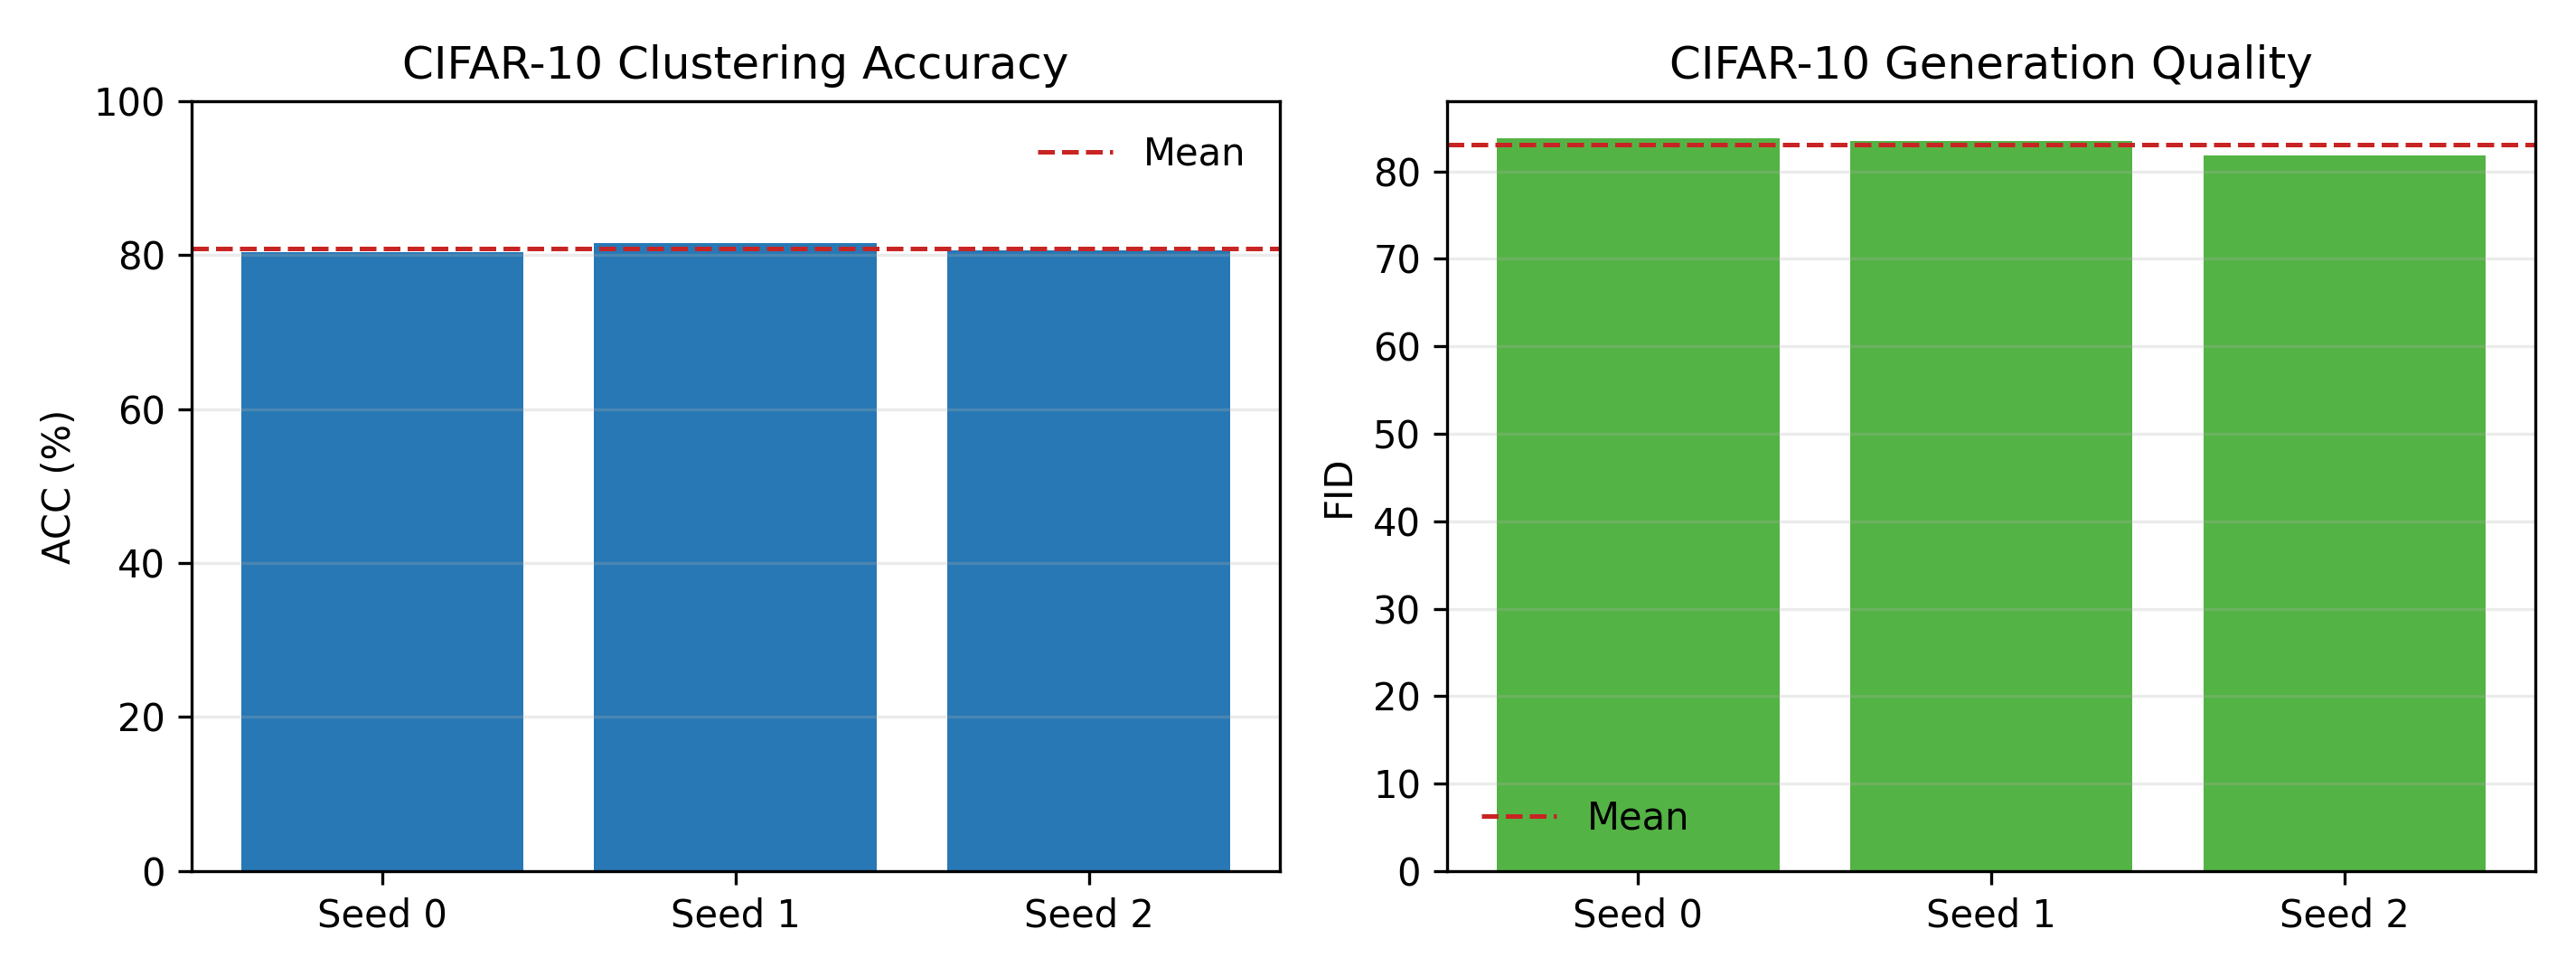
\includegraphics[width=0.95\linewidth]{cifar10_main_metrics.png}
\caption{CIFAR-10 clustering and FID across three \ours{} seeds. Variance is low.}
\label{fig:cifar-main}
\end{figure}

\begin{figure}[t]
\centering
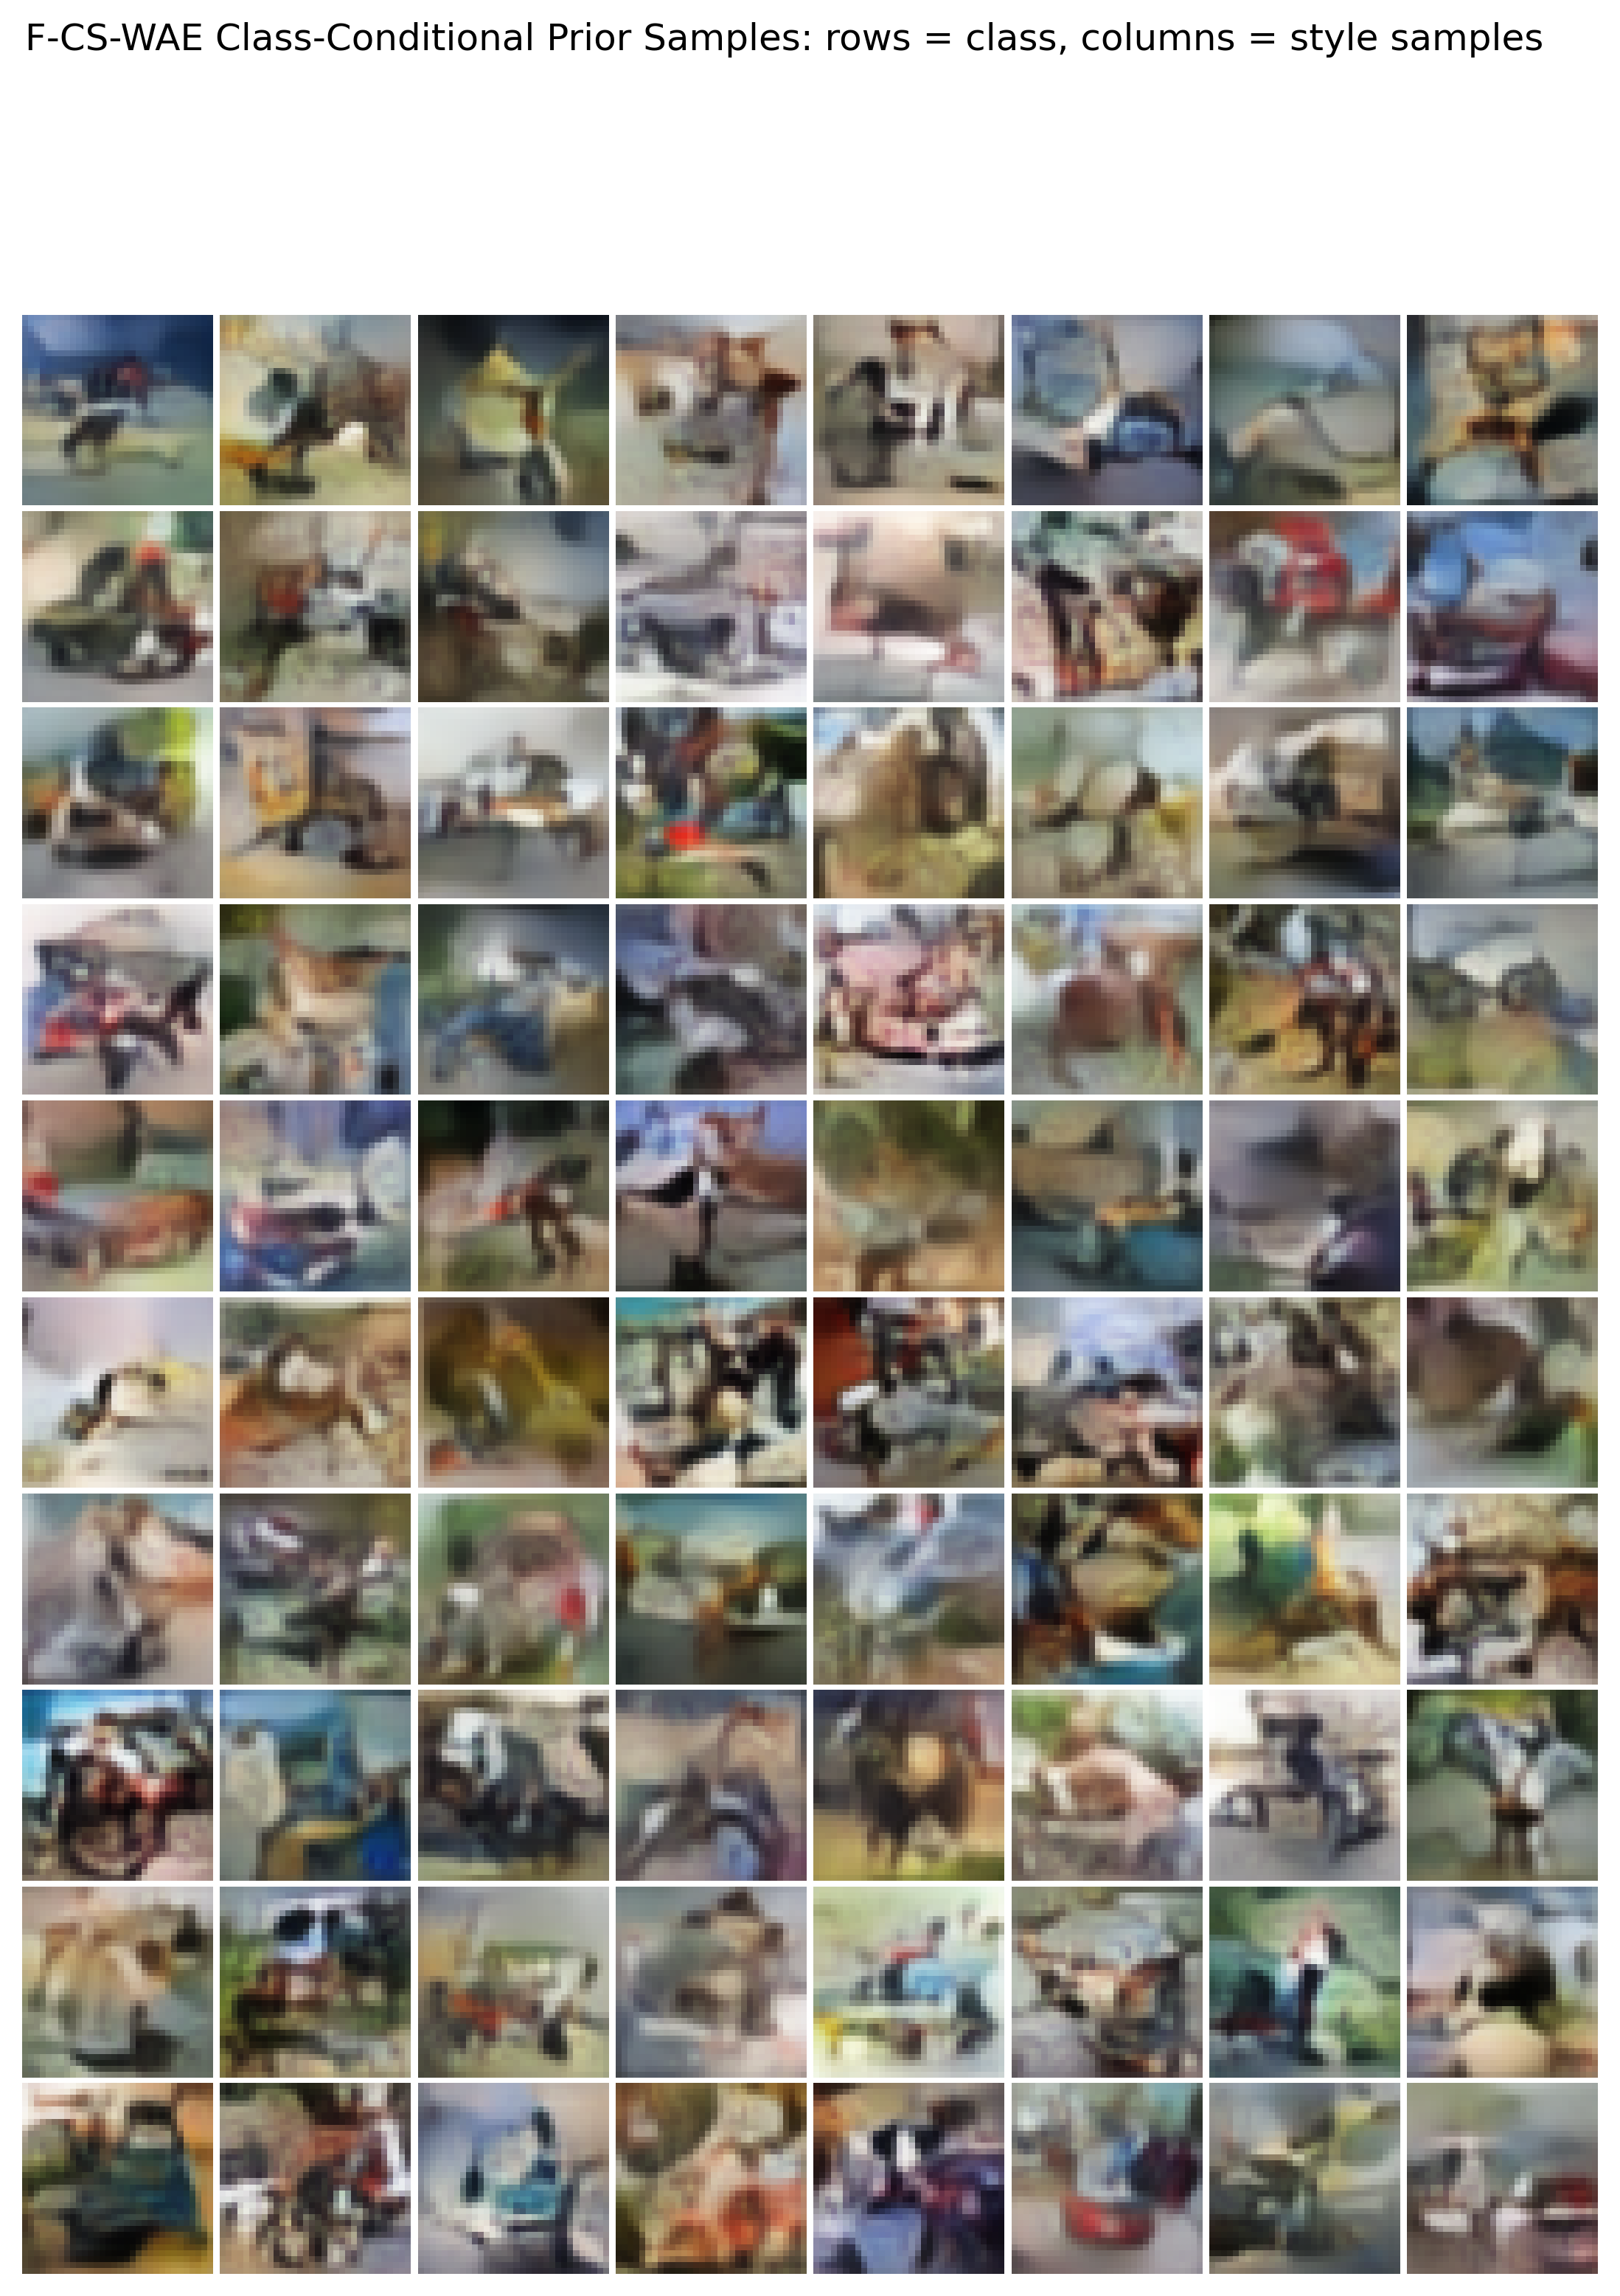
\includegraphics[width=0.95\linewidth]{cifar10_class_prior_grid.png}
\caption{CIFAR-10 class-conditional prior samples (one row per class).}
\label{fig:cifar-samples}
\end{figure}

\begin{figure}[t]
\centering
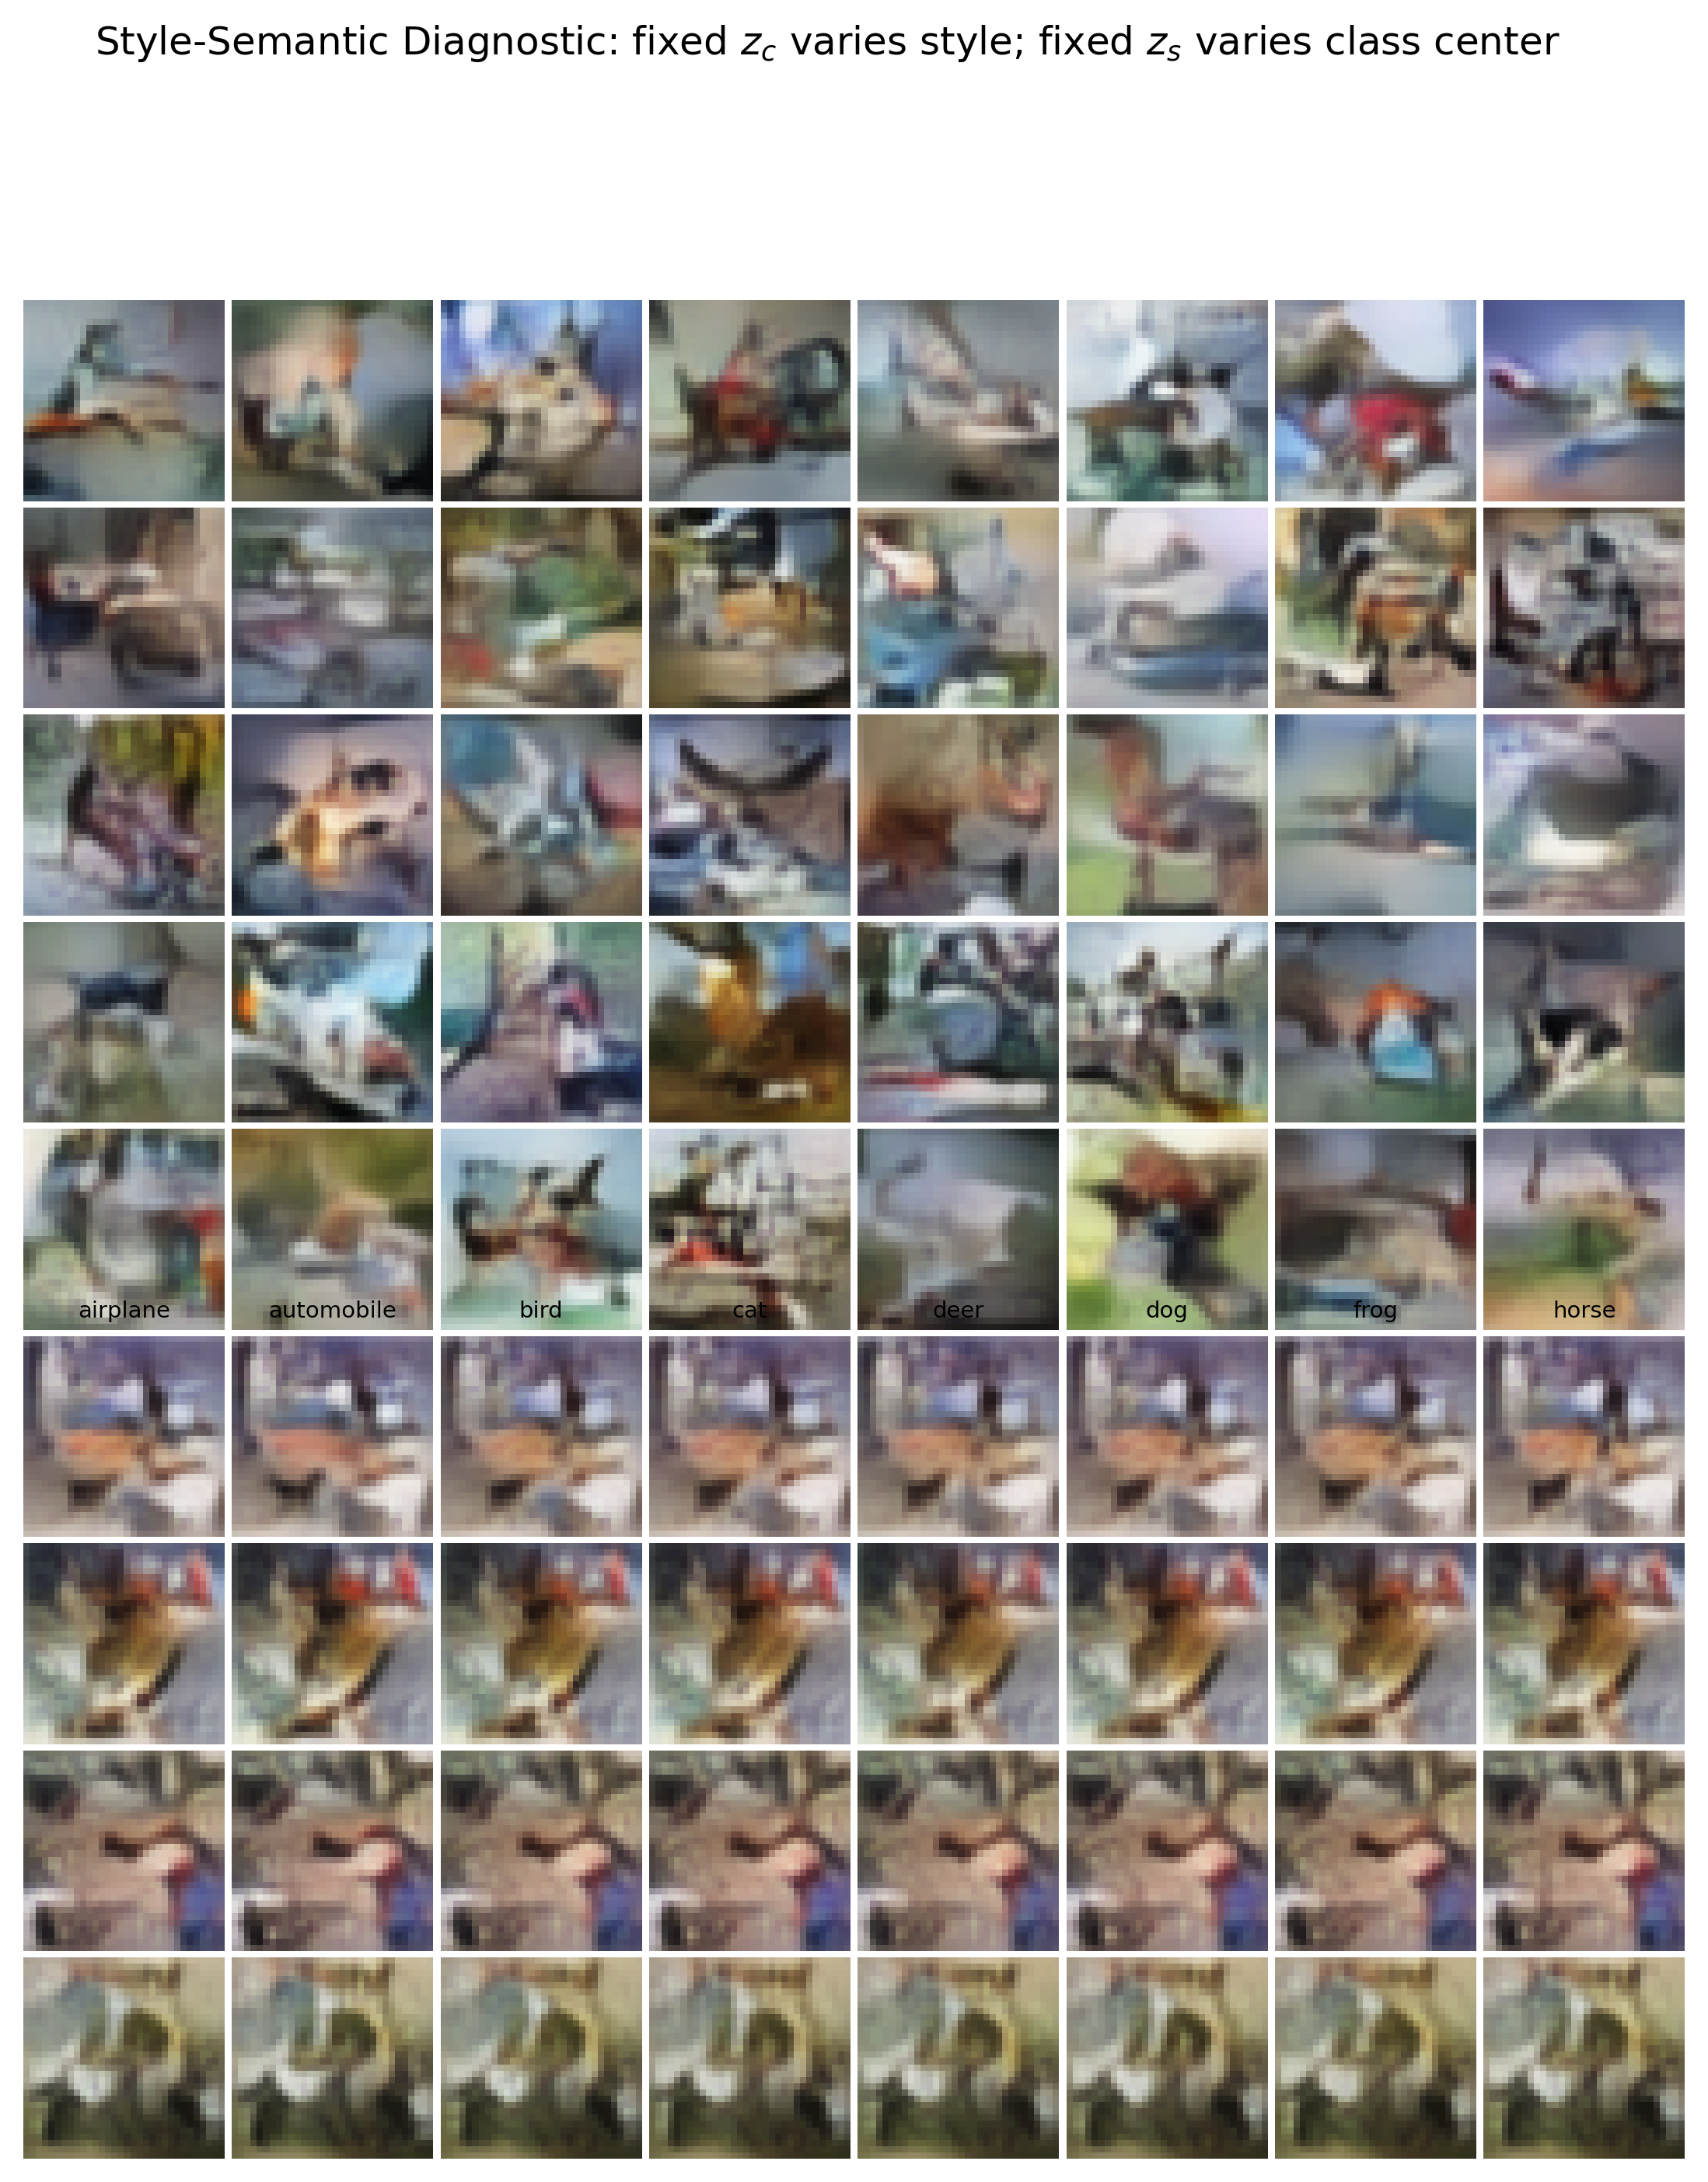
\includegraphics[width=0.95\linewidth]{cifar10_style_semantic_grid.png}
\caption{CIFAR-10 factorization probe.
         Columns: fixed $\zc$, varying $\zs$.
         Rows: fixed $\zs$, varying $\zc$.}
\label{fig:cifar-style}
\end{figure}

\begin{figure}[t]
\centering
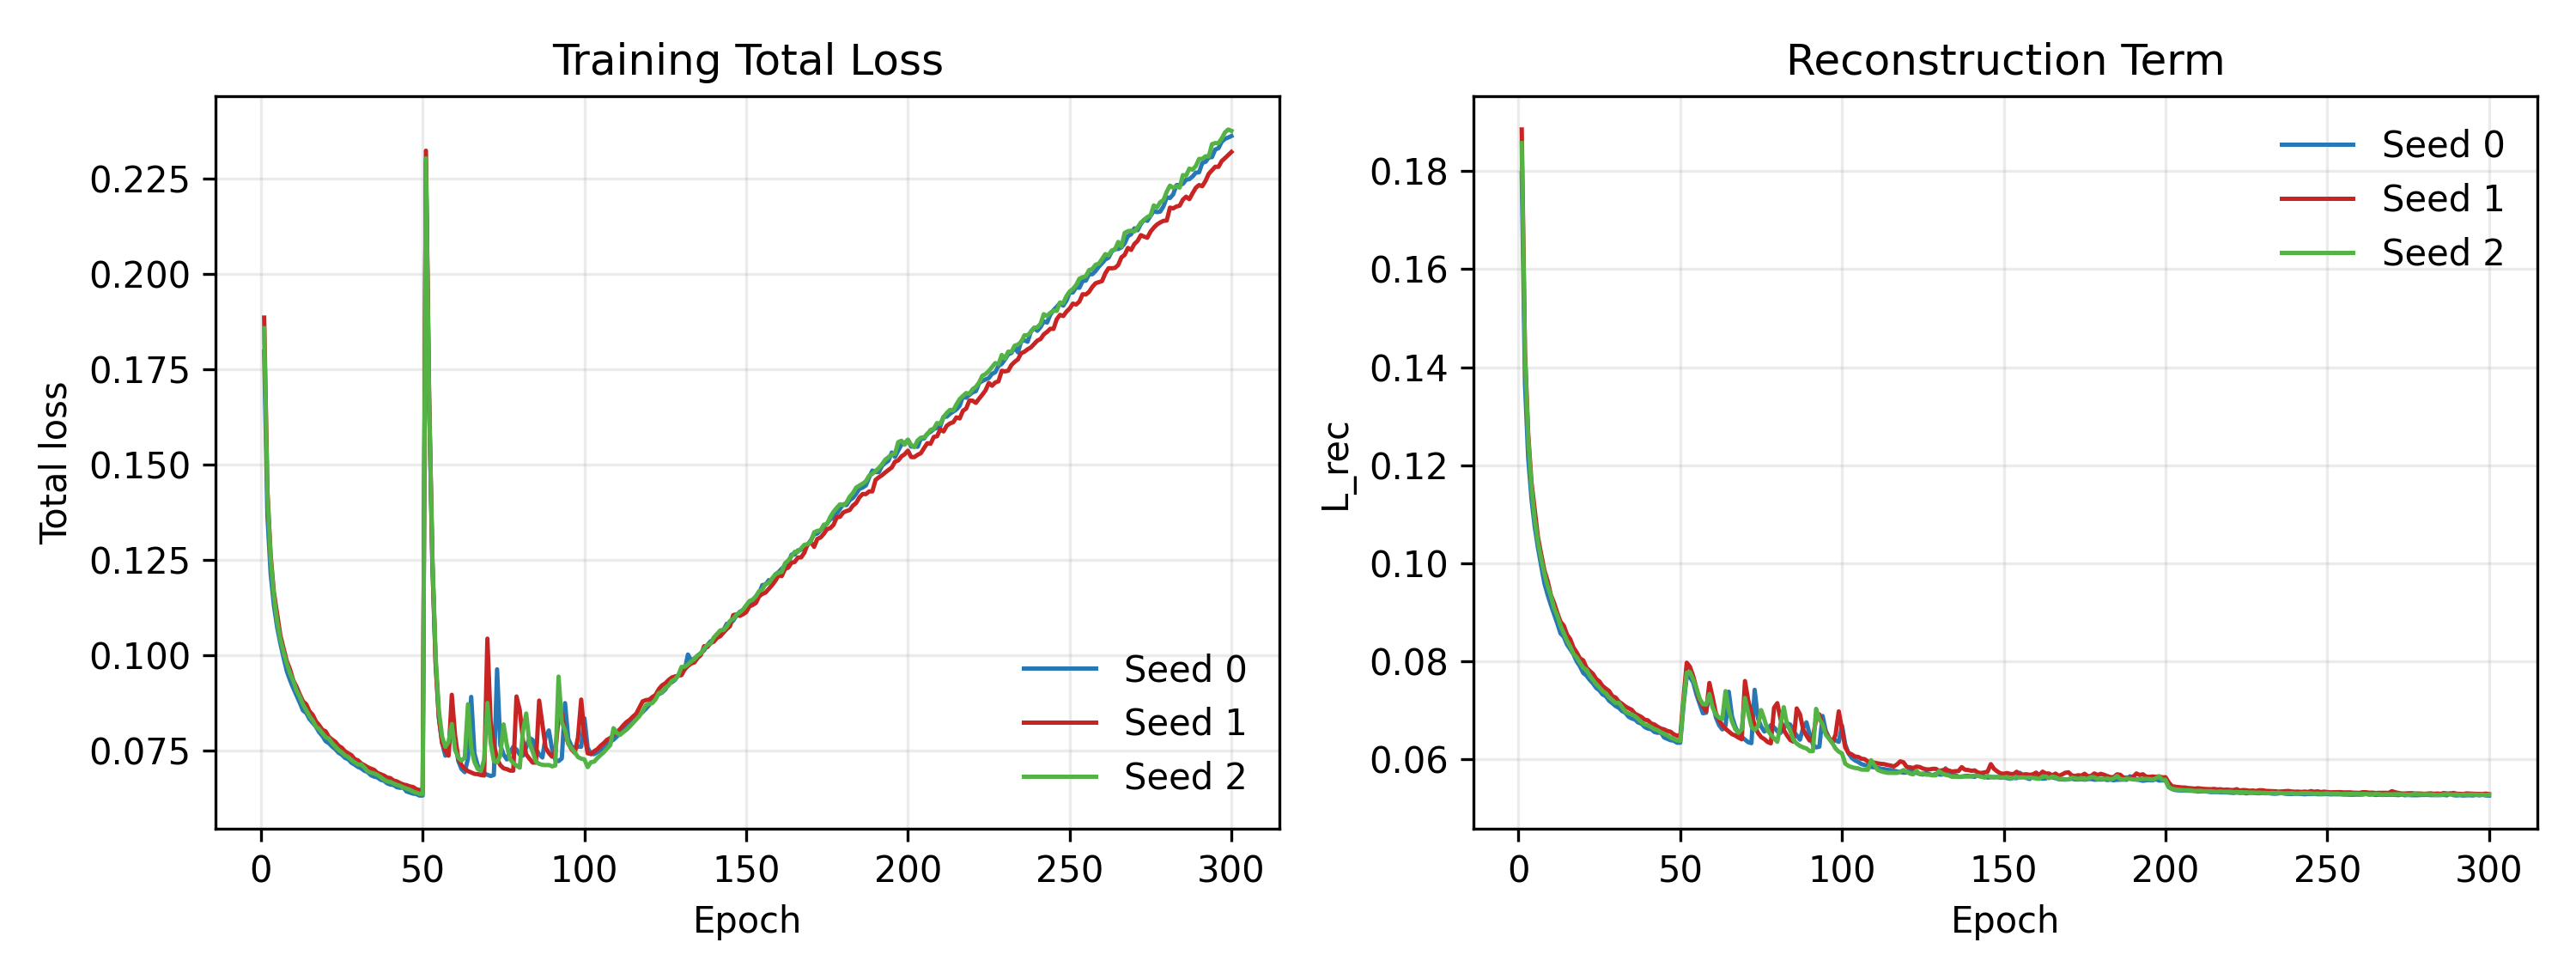
\includegraphics[width=0.95\linewidth]{cifar10_training_curves.png}
\caption{CIFAR-10 training curves. Phase transitions at epochs 50, 100, 200.}
\label{fig:cifar-training}
\end{figure}

\subsection{MNIST: Extreme Conditional Style Leakage}
\label{sec:mnist}

Table~\ref{tab:mnist} shows that \ours{} without per-class style MMD achieves
$99.15\%$ clustering accuracy and SSIM $0.983$ on MNIST, yet class-conditional
generation self-accuracy is only $15\%$.
This is the clearest demonstration of conditional style leakage: near-perfect
performance on all standard metrics coexists with catastrophic generation failure.

\begin{table}[t]
\centering
\caption{MNIST seed-0 comparison.
         \simple{}: single-latent Spherical Cauchy WAE.
         \todo{Expand to 3 seeds; add leakage diagnostic columns.}}
\label{tab:mnist}
\begin{tabular}{lrrrrrrr}
\toprule
Method & ACC & NMI & ARI & SSIM & PSNR & LPIPS & FID \\
\midrule
\simple{}        & 0.8735 & 0.8863 & 0.8411 & 0.8127 & 16.38 & 0.0603 & \textbf{26.95} \\
\textbf{\ours{}} & \textbf{0.9915} & \textbf{0.9758} & \textbf{0.9813}
                 & \textbf{0.9833} & \textbf{26.88} & \textbf{0.0120} & 73.99 \\
\bottomrule
\end{tabular}
\end{table}

\paragraph{Leakage diagnosis.}
We encode 2{,}048 MNIST test images and measure the style latent.
Global MMD to $\mathcal{N}(0,I)$ is $0.0017$---the aggregate regularizer appears
to have succeeded.
Yet the inter-class style separation is $\Delta_{\mathrm{inter}}=6.25$, far above
zero, and a linear probe trained on $\zs$ achieves $100.0\%$ accuracy
(chance: $10\%$; computed via \texttt{scripts/compute\_leakage\_diagnostics.py}
on the MNIST checkpoint).
Figure~\ref{fig:style-diagnostic} visualizes the class-conditional structure.

The formal gap from Proposition~\ref{prop:marginal-not-sufficient} is directly
illustrated here: the marginal is $\mathcal{N}(0,I)$-like, but each conditional
$q(\zs\mid y{=}k)$ has a class-specific mean, and the decoder has learned to exploit
these class-specific means.

\begin{figure}[t]
\centering
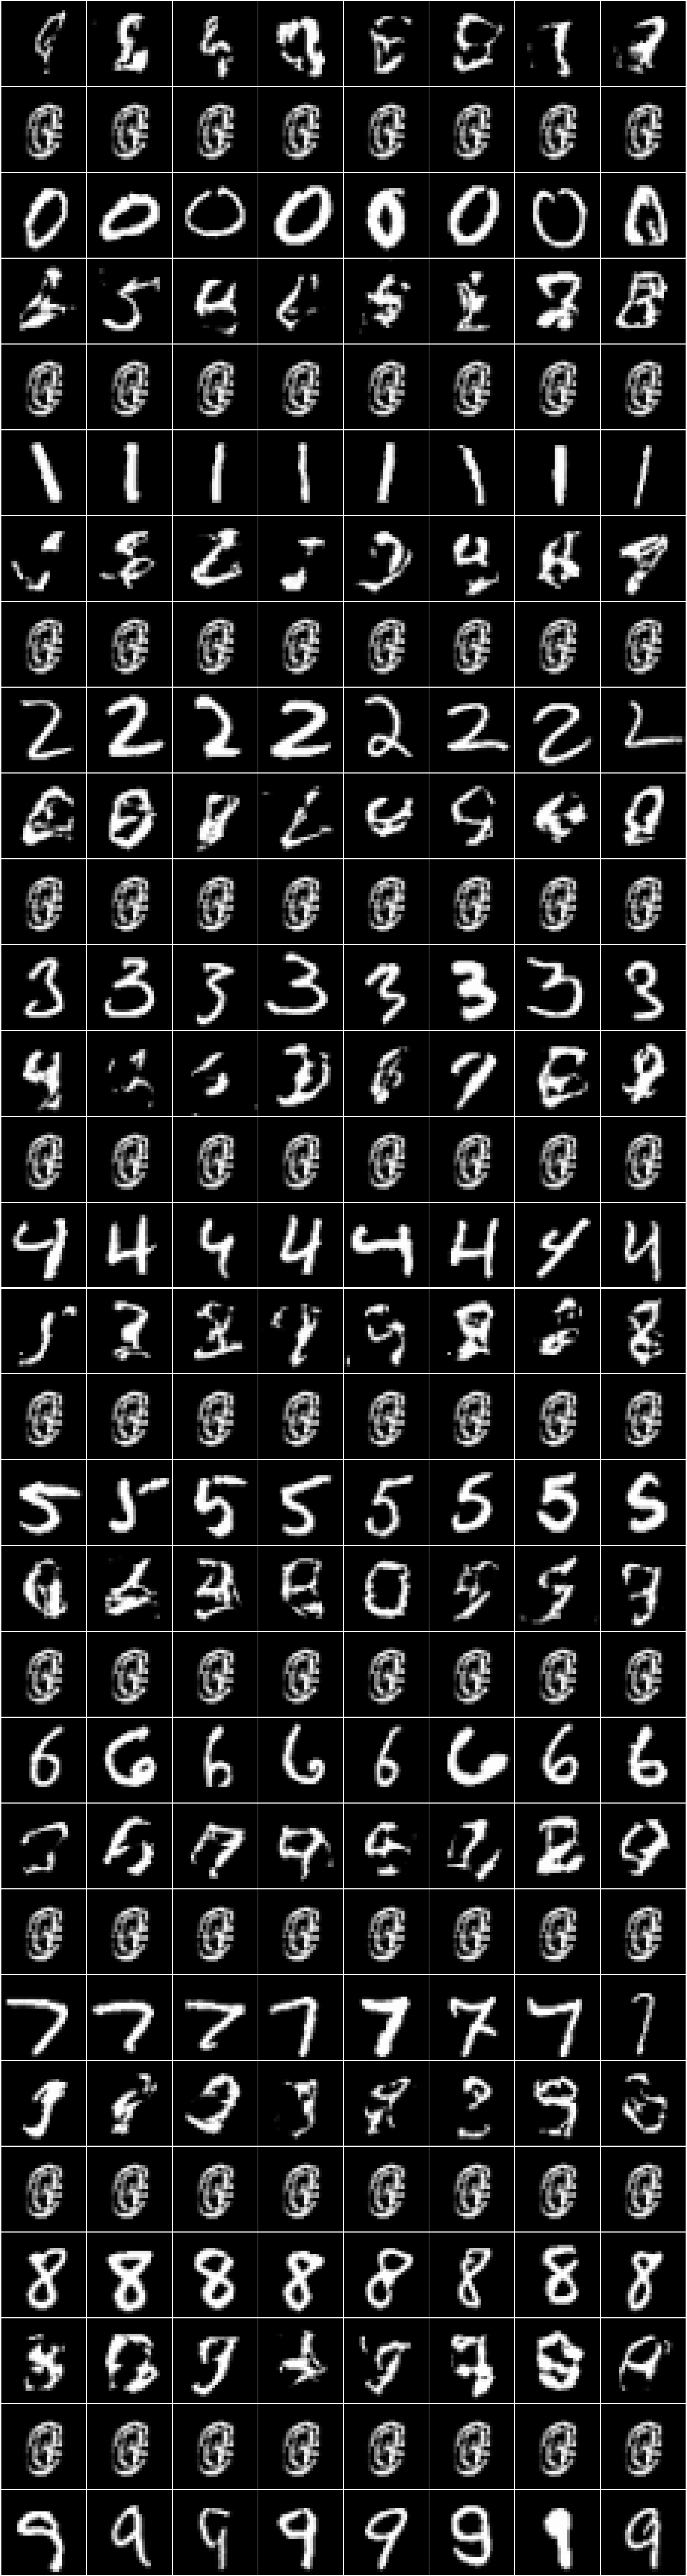
\includegraphics[width=0.88\linewidth]{mnist_style_prior_diagnostic.png}
\caption{MNIST style latent diagnostic.
         Global MMD $\approx 0.0017$, yet class-conditional means are clearly
         separated ($\Delta_{\mathrm{inter}}=6.25$).}
\label{fig:style-diagnostic}
\end{figure}

\subsection{Representation-Aware Sampling Strategies}
\label{sec:sampling}

Table~\ref{tab:sampling} evaluates four style sampling strategies on the
trained MNIST checkpoint, demonstrating that the failure is in the sampling
distribution and that any class-conditional correction restores generation.

\begin{table}[t]
\centering
\caption{MNIST generation under representation-aware style sampling strategies.
         All strategies sample $\zc$ from the Spherical Cauchy class prior.
         Self-ACC = fraction of generated images classified to the intended class.
         Confidence = mean classifier probability at the predicted class.
         Diversity = mean pixel standard deviation across samples.}
\label{tab:sampling}
\begin{tabular}{lrrr}
\toprule
Style sampling $\zs$ & Self-ACC $\uparrow$ & Confidence $\uparrow$ & Diversity $\uparrow$ \\
\midrule
Global Gaussian $\mathcal{N}(0,I)$           & 0.150 & 0.934 & 0.151 \\
Class mean $\bar\mus^{(k)}$                  & 1.000 & 1.000 & 0.132 \\
Class diagonal Gaussian, $\tau=0.50$         & 1.000 & 0.990 & 0.139 \\
Class diagonal Gaussian, $\tau=0.25$         & \textbf{1.000} & \textbf{1.000} & 0.135 \\
Empirical style bank                         & 1.000 & 1.000 & \textbf{0.182} \\
\bottomrule
\end{tabular}
\end{table}

The key result: any form of class conditioning on $\zs$ restores perfect self-accuracy.
The class-conditional diagonal Gaussian with $\tau=0.25$ is the recommended
generation prior: true parametric sampler, perfect class consistency, preserves
diversity over a point estimate.

\begin{figure*}[t]
\centering
\begin{subfigure}[t]{0.24\linewidth}
  \centering
  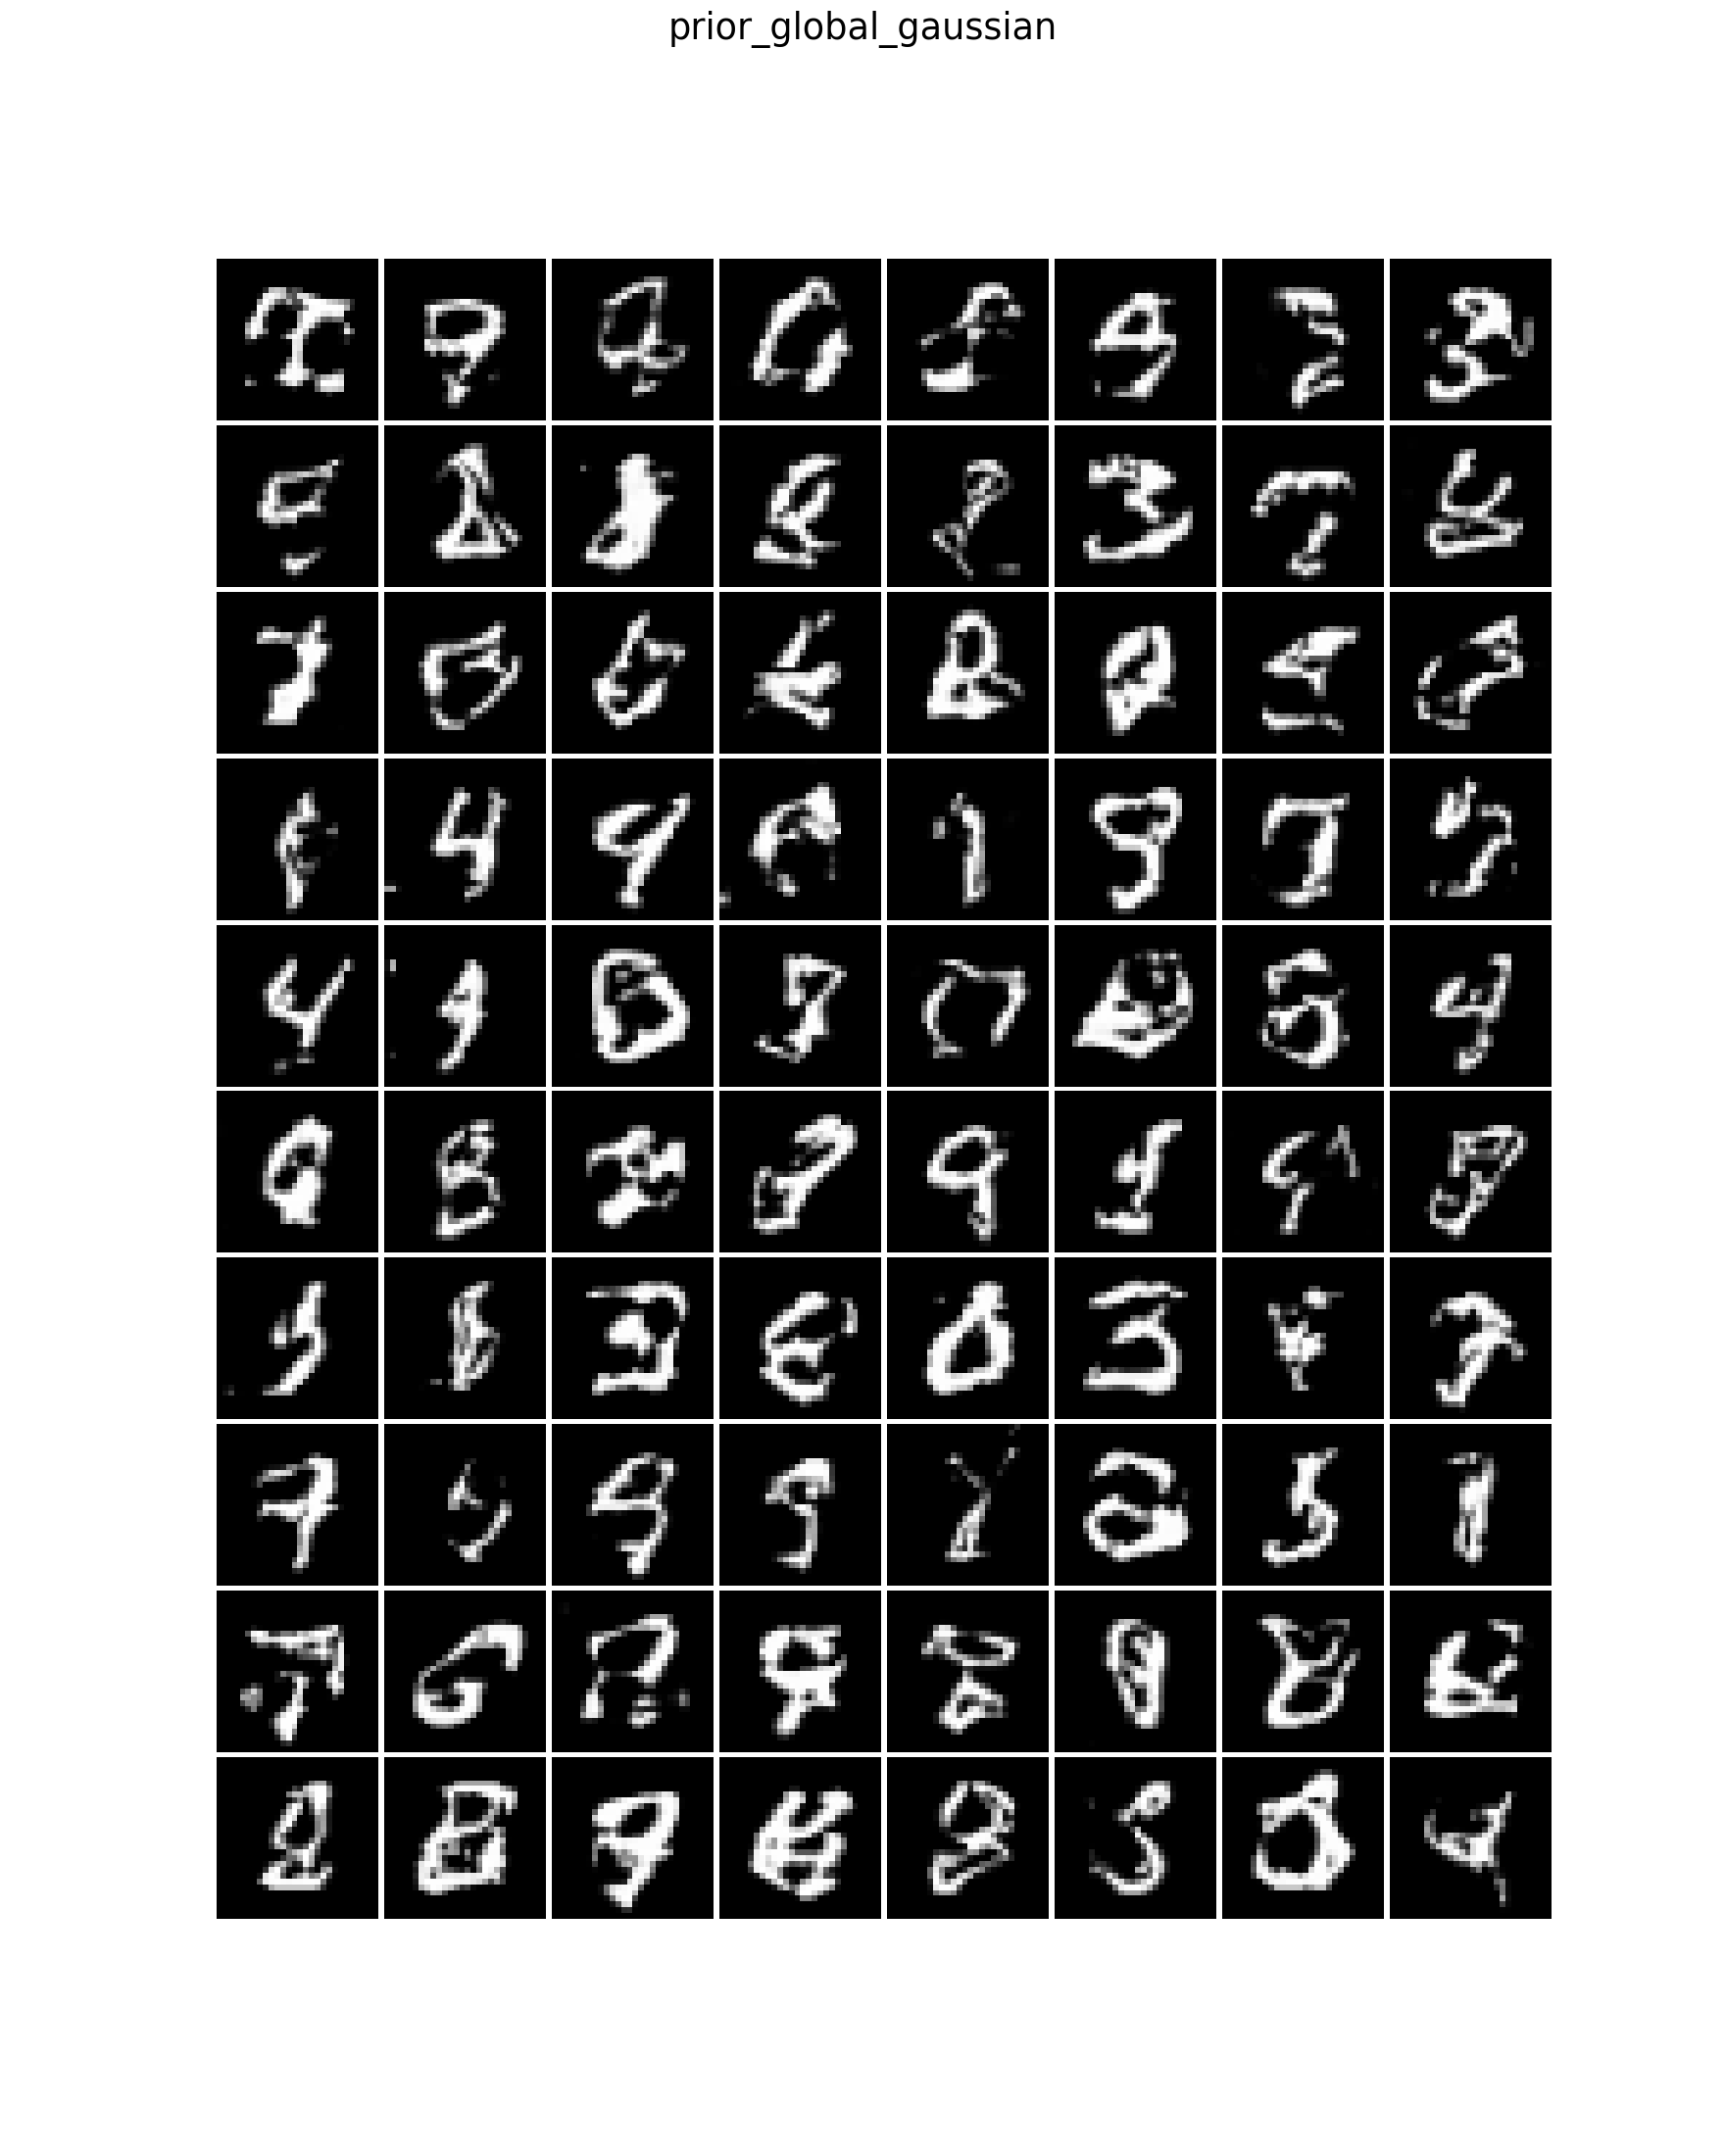
\includegraphics[width=\linewidth]{mnist_sampling_global_gaussian.png}
  \caption{Global Gaussian\\(self-ACC: 15\%)}
\end{subfigure}
\hfill
\begin{subfigure}[t]{0.24\linewidth}
  \centering
  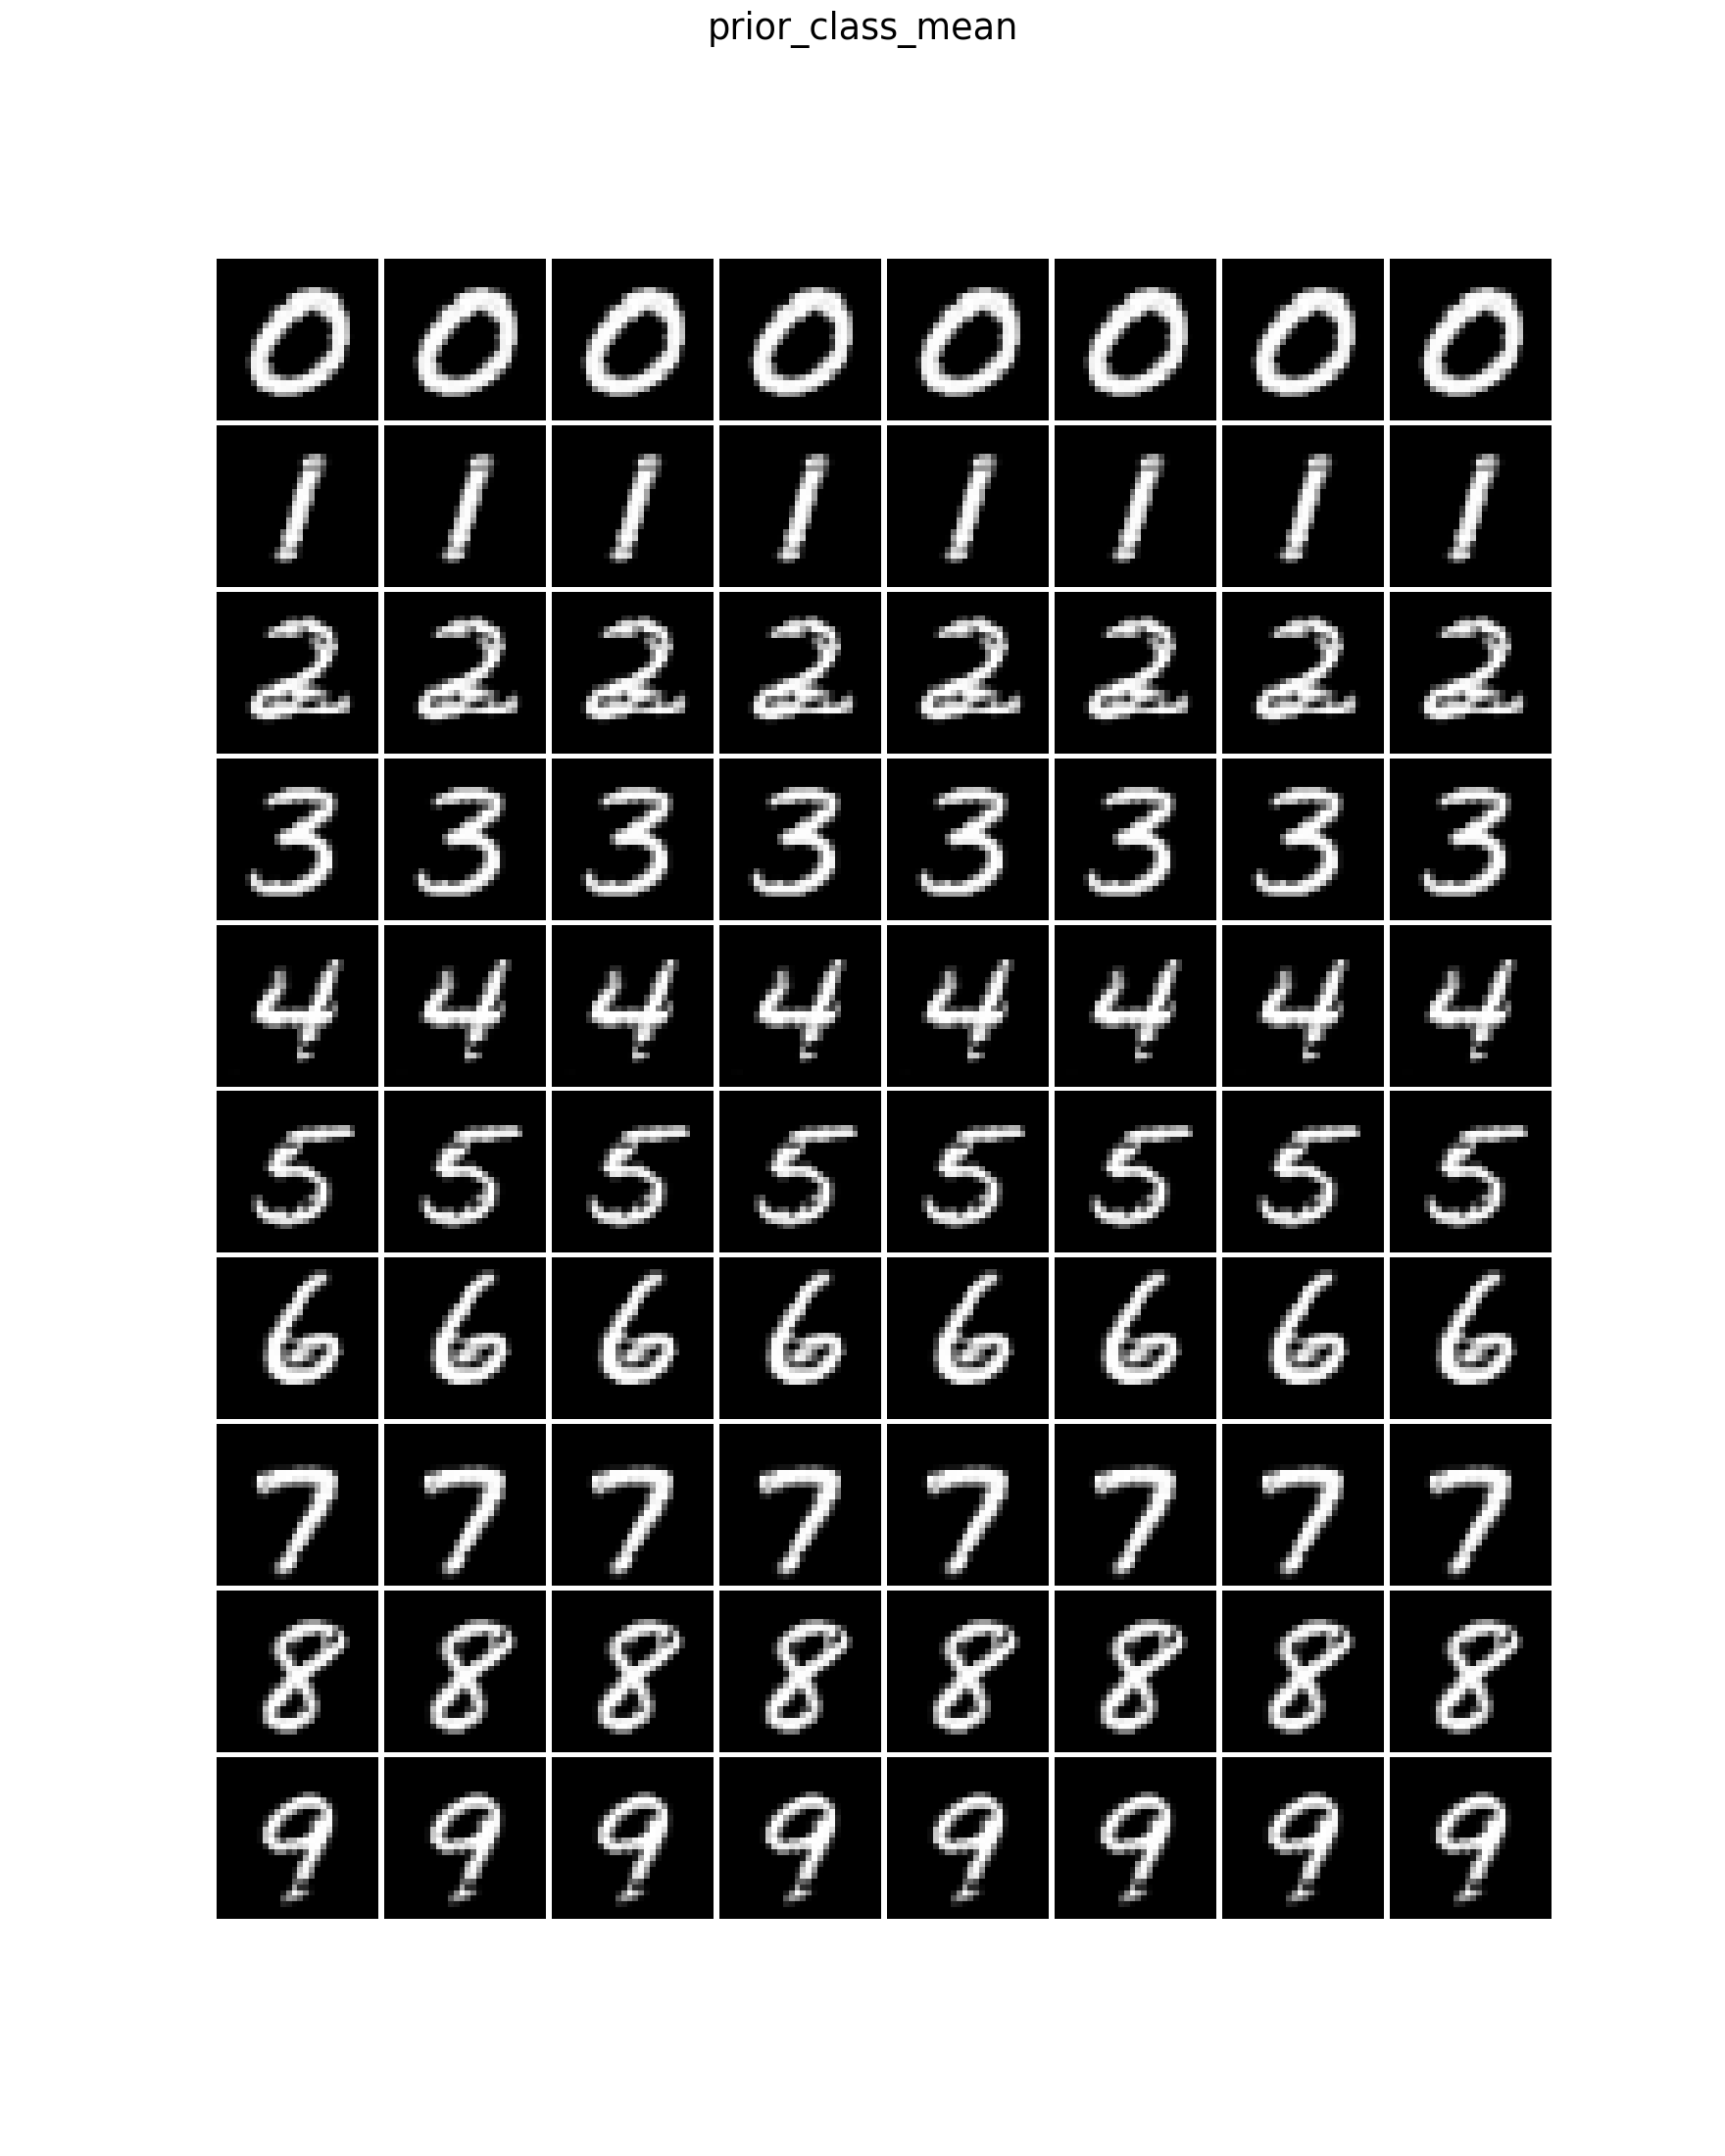
\includegraphics[width=\linewidth]{mnist_sampling_class_mean.png}
  \caption{Class mean style\\(self-ACC: 100\%)}
\end{subfigure}
\hfill
\begin{subfigure}[t]{0.24\linewidth}
  \centering
  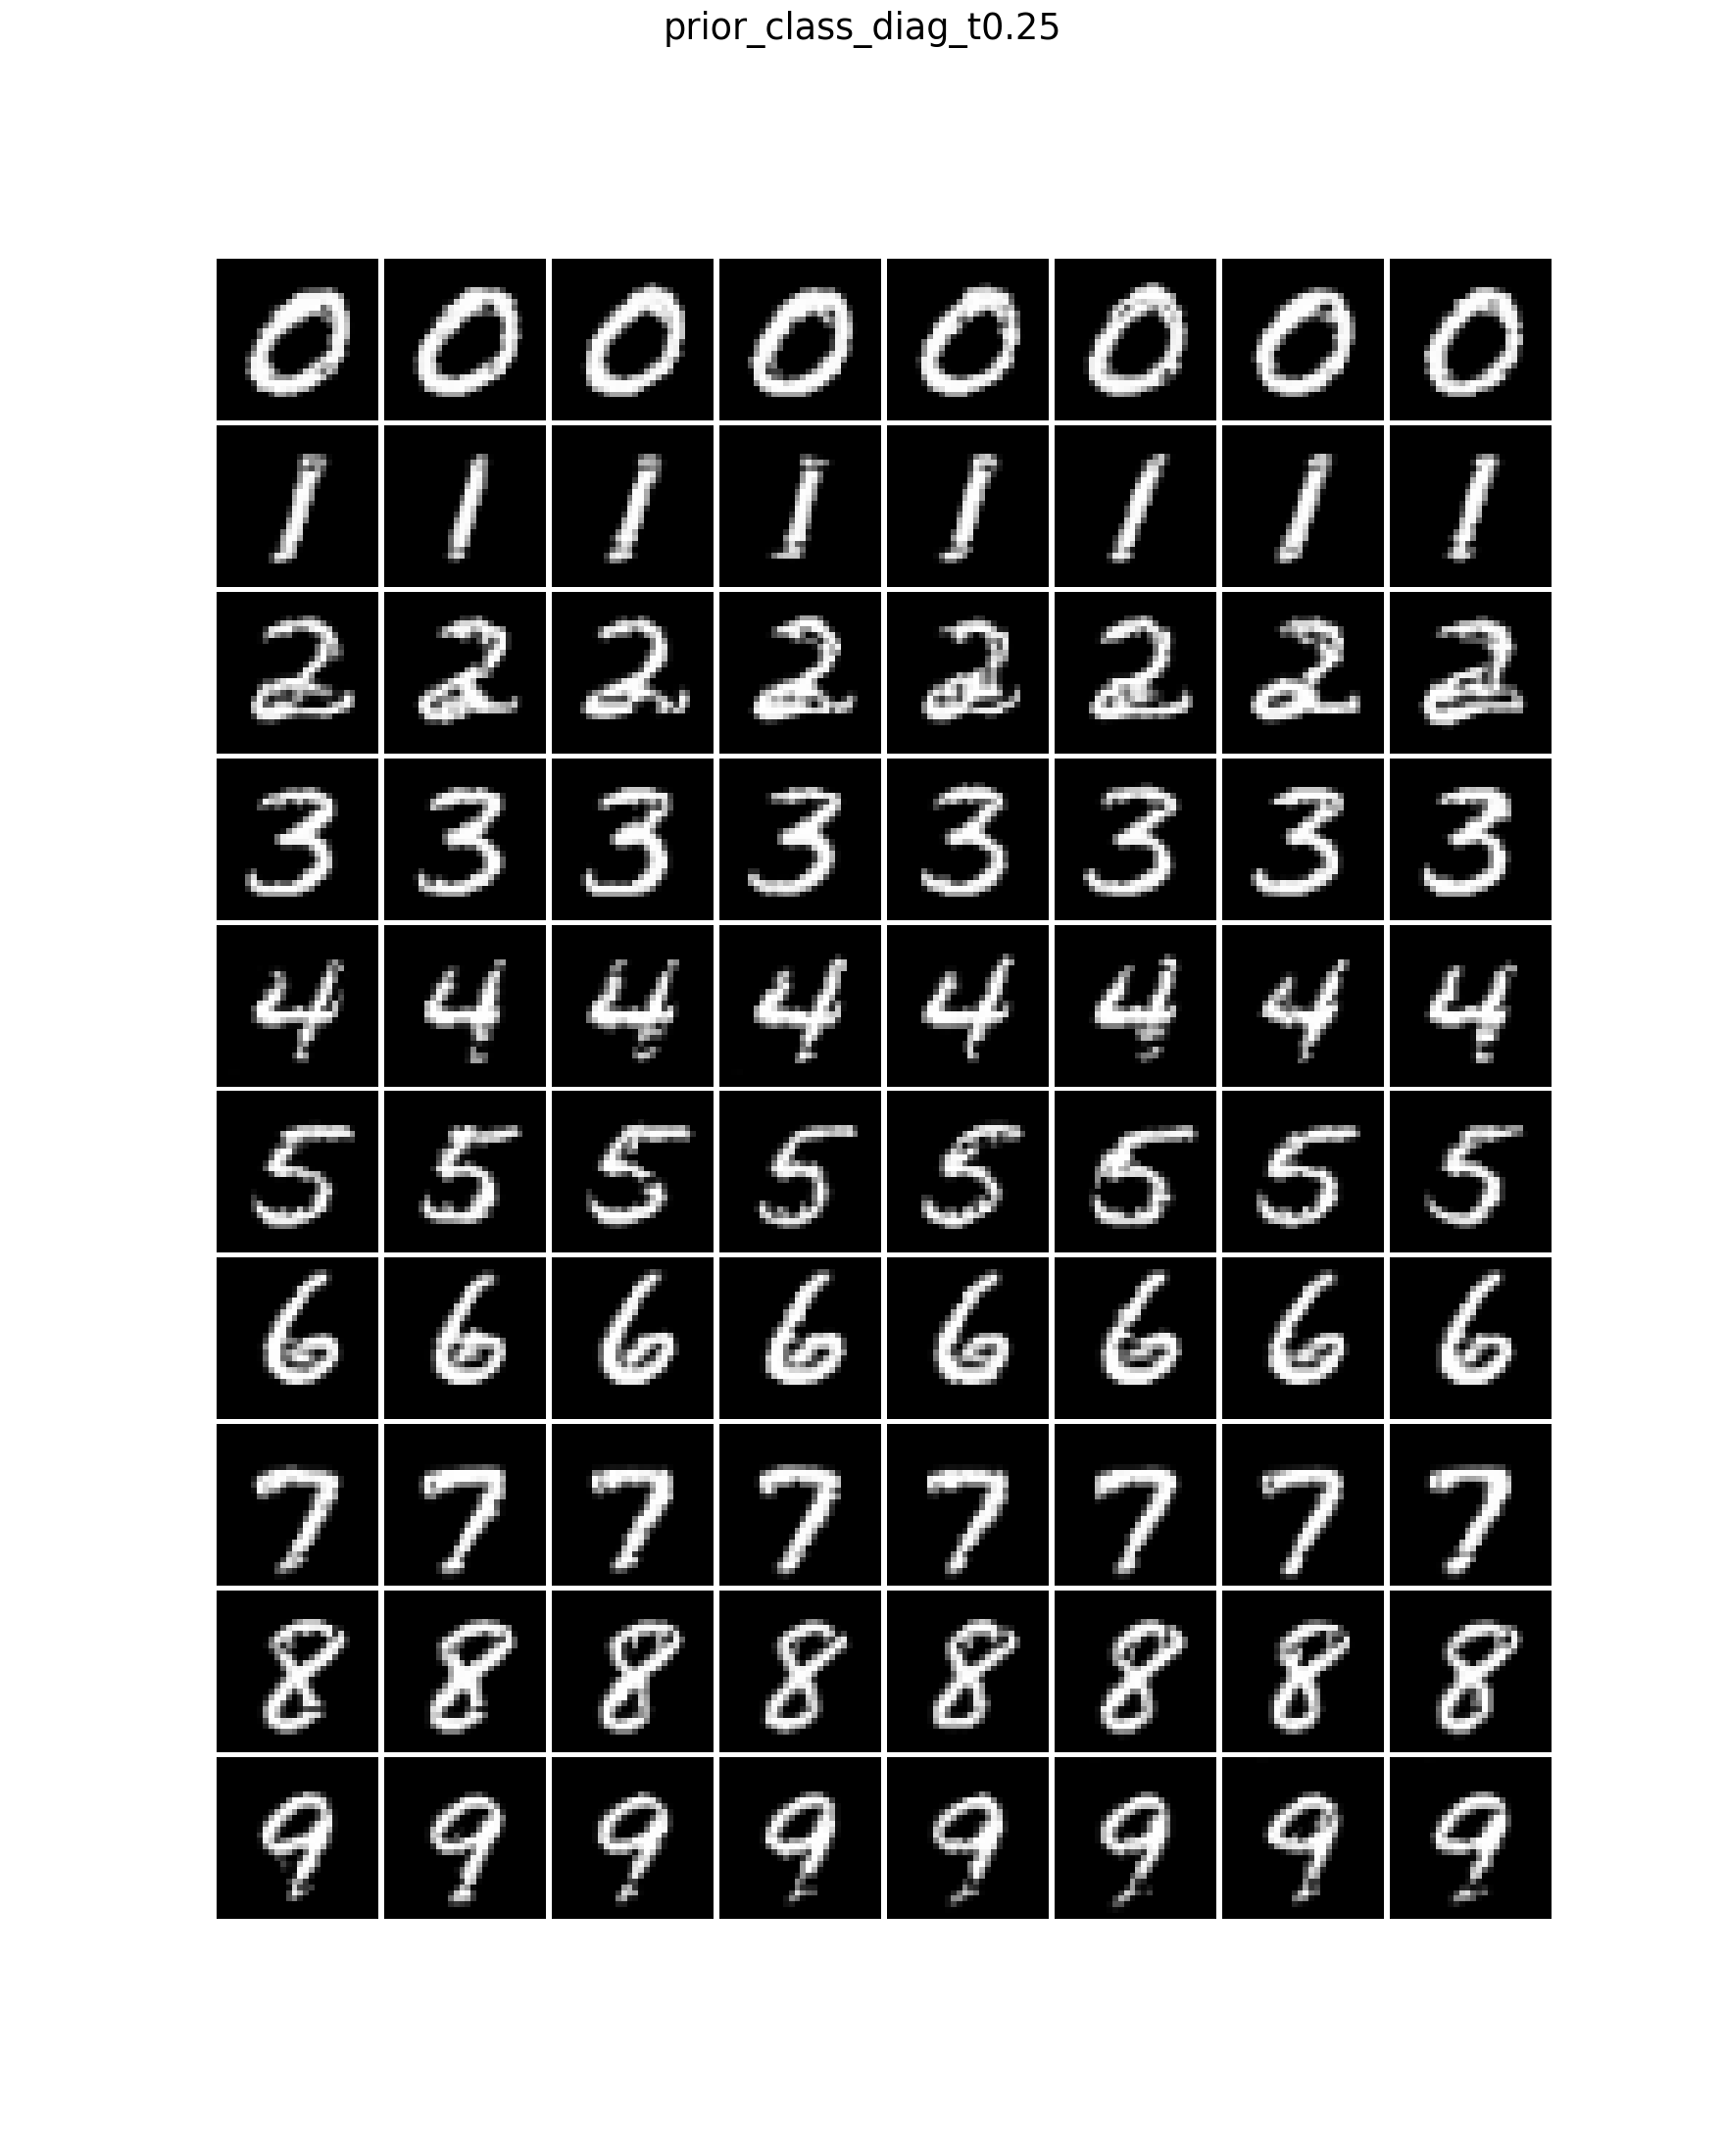
\includegraphics[width=\linewidth]{mnist_sampling_class_diag_t025.png}
  \caption{Class diag., $\tau{=}0.25$\\(self-ACC: 100\%)}
\end{subfigure}
\hfill
\begin{subfigure}[t]{0.24\linewidth}
  \centering
  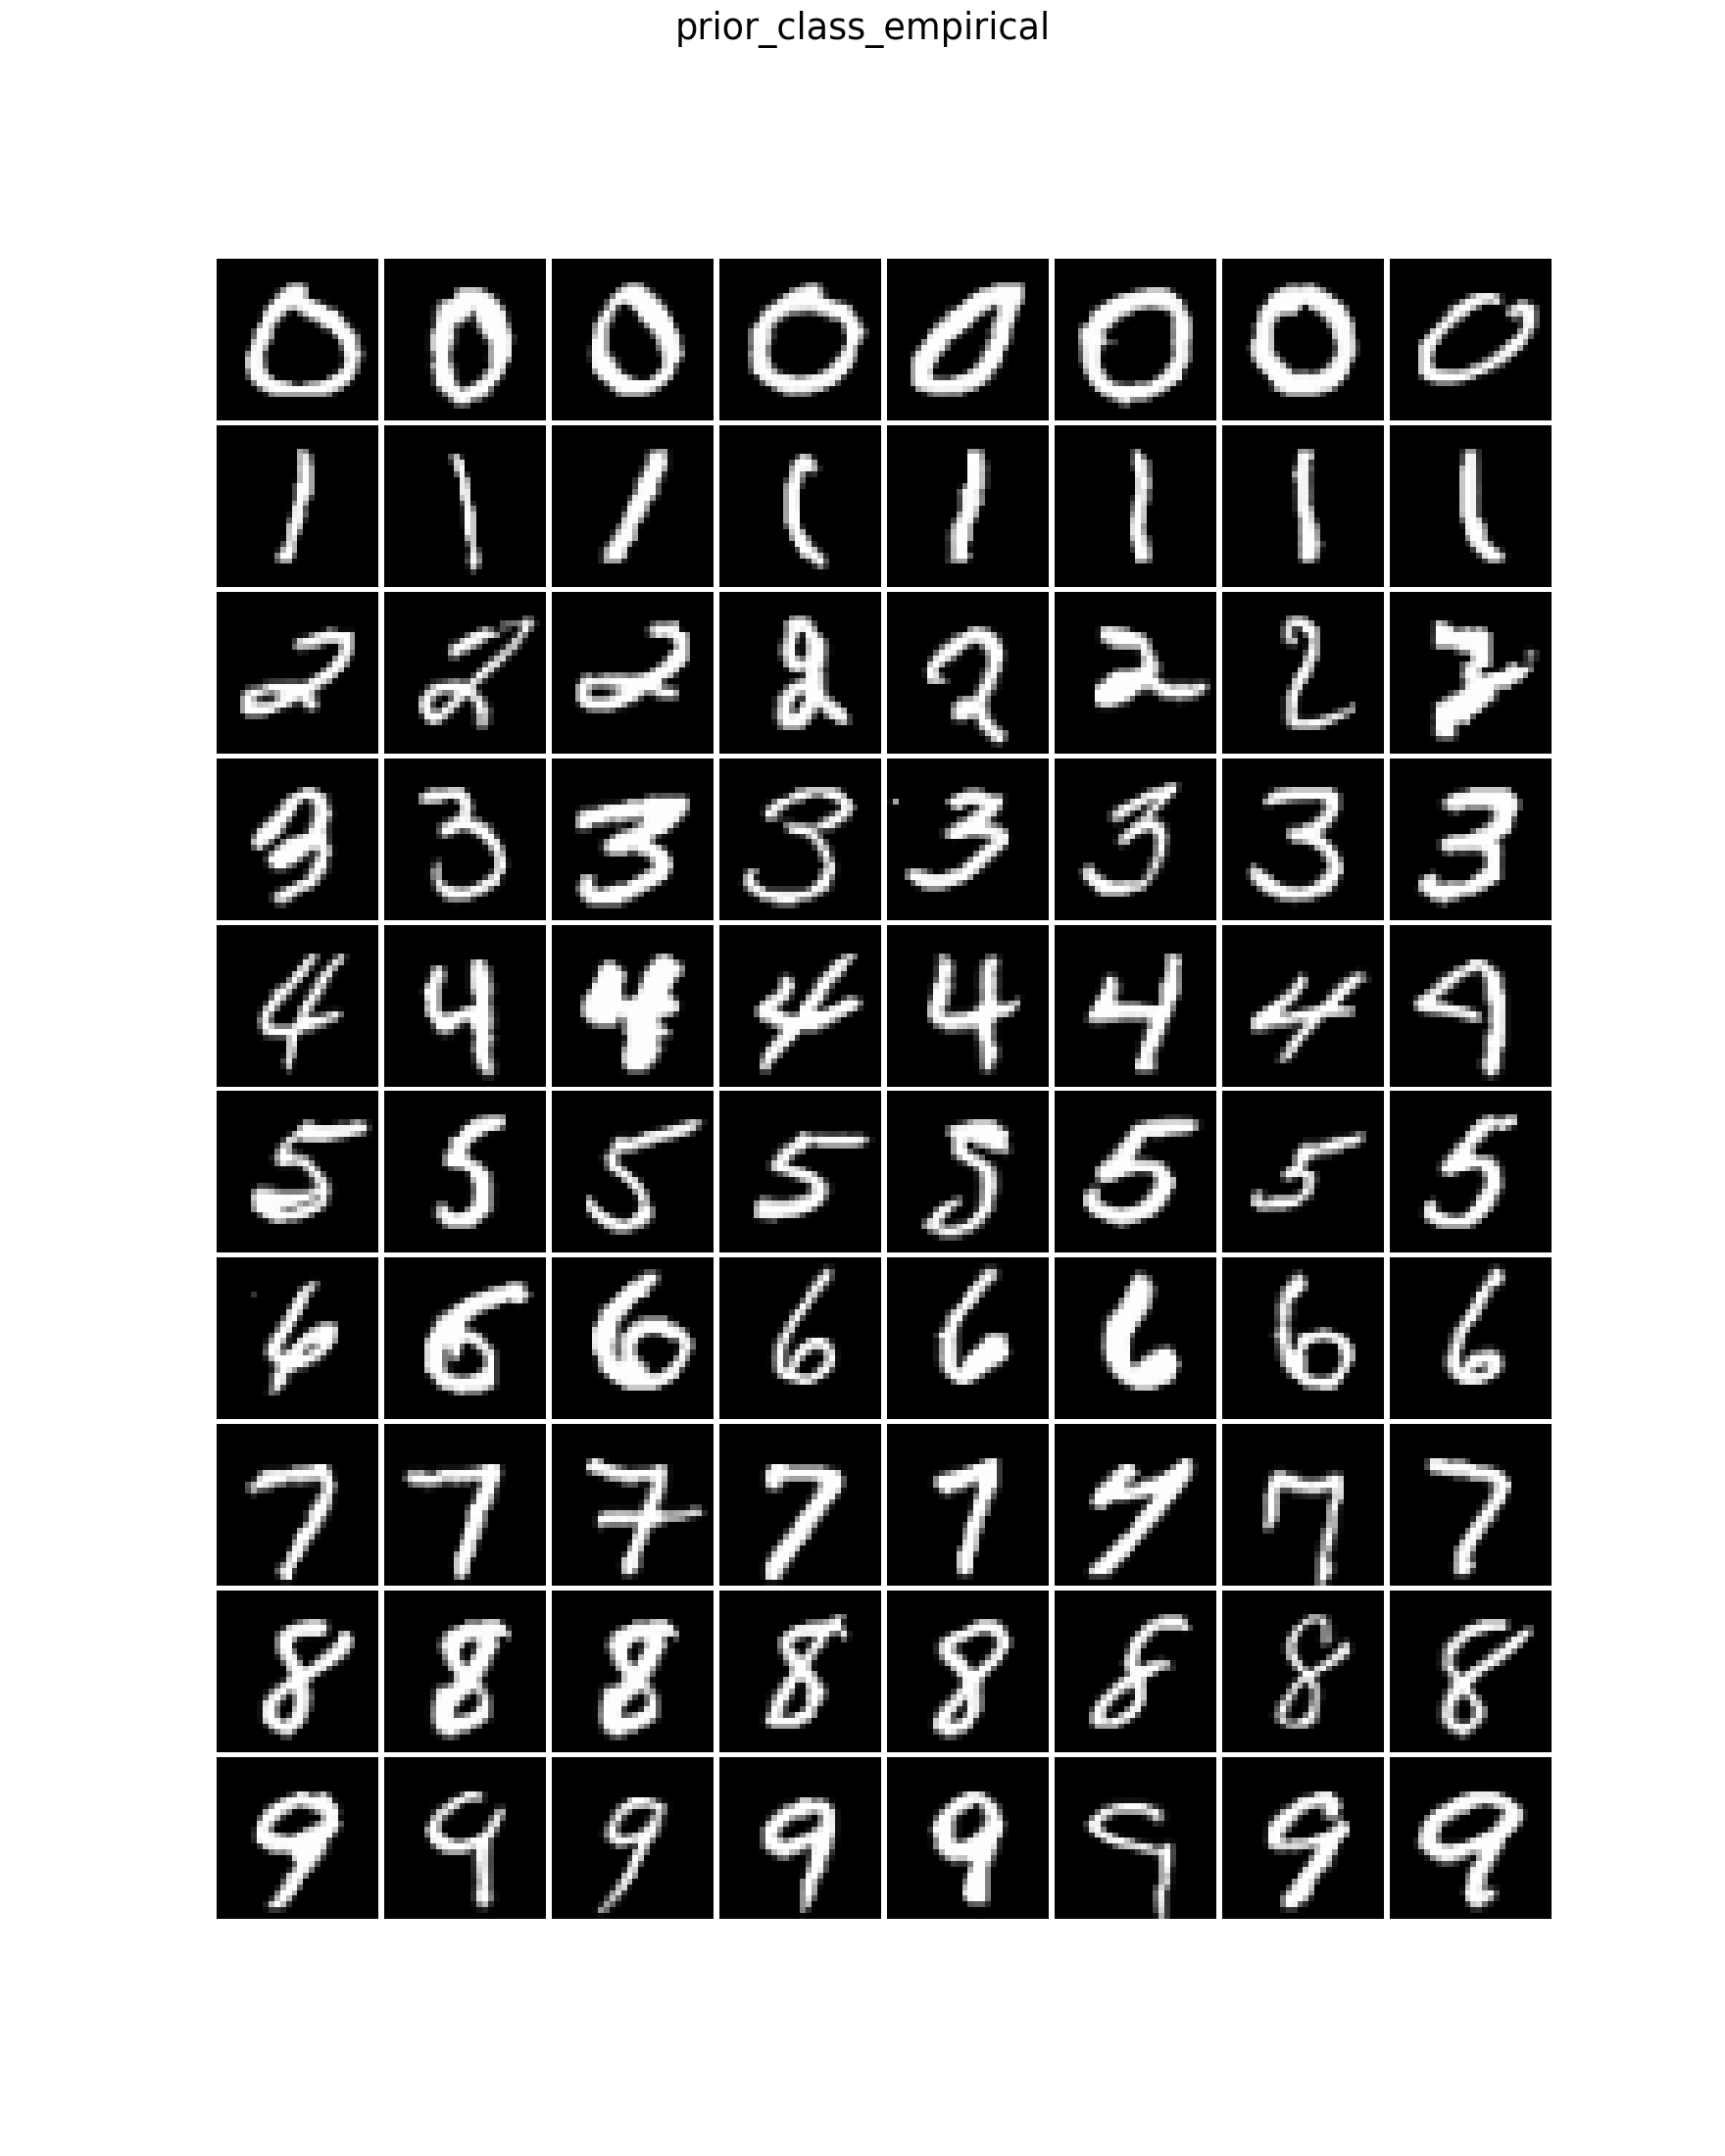
\includegraphics[width=\linewidth]{mnist_sampling_class_empirical.png}
  \caption{Empirical style bank\\(self-ACC: 100\%)}
\end{subfigure}
\caption{MNIST generation under representation-aware style sampling.
         Global Gaussian produces shapeless images; all class-conditional strategies
         restore correct digit identity.}
\label{fig:sampling-strategies}
\end{figure*}

\subsection{Ablation Study}
\label{sec:ablations}

Table~\ref{tab:ablations} reports CIFAR-10 clustering and leakage diagnostics for
key design choices.

\begin{table}[t]
\centering
\caption{CIFAR-10 ablations. Seed 0.
         ``$\Delta_{\mathrm{inter}}$'' is measured on the CIFAR-10 checkpoint itself
         (not MNIST) via \texttt{scripts/compute\_leakage\_diagnostics.py}.
         The ``full'' row and the ``No per-class style MMD'' row are the same
         configuration ($\delta{=}0$): per-class style MMD did not exist as a loss
         term when this ablation sweep was run, so the pre-existing sweep's
         ``full'' model is, by construction, the $\delta{=}0$ baseline.
         \todo{Remaining variants (no $\zs$, no class MMD, no aux classifier,
         Gaussian/vMF prior) not yet re-run under the current codebase.}}
\label{tab:ablations}
\renewcommand{\arraystretch}{1.05}
\begin{tabular}{lcccc}
\toprule
Variant & ACC & NMI & ARI & $\Delta_{\mathrm{inter}}$ \\
\midrule
\ours{} (full, seed 0, $\delta{=}0$)      & 0.8149 & 0.6622 & 0.6438 & 4.19 \\
\ours{} + per-class style MMD ($\delta{=}1$) & 0.8000 & 0.6386 & 0.6177 & 1.28 \\
\midrule
\emph{Remove components (relative to $\delta{=}0$ full model):} & & & & \\
\quad No $\zs$ (semantic-only)            & \todo{} & \todo{} & \todo{} & N/A \\
\quad No class MMD ($\alpha{=}0$)         & \todo{} & \todo{} & \todo{} & \todo{} \\
\quad No per-class style MMD ($\delta{=}0$)& \multicolumn{4}{l}{(same as ``full, seed 0'' row above)} \\
\quad No auxiliary classifier ($\eta{=}0$)& \todo{} & \todo{} & \todo{} & \todo{} \\
\midrule
\emph{Prior geometry:}                    & & & & \\
\quad Gaussian semantic prior             & \todo{} & \todo{} & \todo{} & \todo{} \\
\quad vMF semantic prior                  & \todo{} & \todo{} & \todo{} & \todo{} \\
\bottomrule
\end{tabular}
\end{table}

\textbf{Effect of per-class style MMD.}
Contrary to our initial expectation, adding $\mathcal{L}_{\mathrm{style\text{-}cls}}$
does \emph{not} drive $\Delta_{\mathrm{inter}}$ fully to $0$, and it is not free of
cost on clustering quality.
On CIFAR-10, the effect is close to the hoped-for outcome: clustering accuracy is
essentially preserved ($0.8149\to0.8000$ ACC, within normal seed variance;
Table~\ref{tab:cifar-main}), $\Delta_{\mathrm{inter}}$ drops by $67\%$
($4.19\to1.28$), and FID under naive global-Gaussian sampling improves
($80.51\to74.42$).
On MNIST the leakage reduction is larger in relative terms
($\Delta_{\mathrm{inter}}$ drops by $77\%$, $6.27\to1.46$; naive-sampling FID improves
sharply, $73.99\to43.36$; self-accuracy rises from $15\%$ to $70\%$), but clustering
accuracy drops substantially ($99.15\%\to85.92\%$ ACC).
We interpret this as evidence that on MNIST---where classes are visually
uniform---the style variable had been carrying class-discriminative information
that the semantic variable alone did not fully capture; suppressing that
information via $\mathcal{L}_{\mathrm{style\text{-}cls}}$ removes a source of
leakage but also removes a signal the clustering pipeline (K-means on $\muc$) was
implicitly benefiting from, even though $\zs$ is never used at clustering time.
This is consistent with the mechanism in Section~\ref{sec:mechanism}: the more a
dataset forces class information into $\zs$, the more a regularizer that
suppresses it can perturb training dynamics elsewhere in the model.
Reaching self-accuracy $\approx 100\%$ still requires combining per-class style MMD
with the post-hoc class-conditional style prior (Section~\ref{sec:sampling}); neither
remedy alone eliminates the failure on MNIST, though either substantially reduces it.

% ============================================================
\section{Discussion}
% ============================================================

\paragraph{Why CIFAR-10 is milder than MNIST.}
On CIFAR-10, naive prior sampling yields FID $83.04$ and visually plausible images.
We hypothesize that CIFAR-10's high intra-class visual diversity (pose, color,
background, texture) causes $\zs$ to carry primarily semantically neutral variation,
weakening conditional style dependence.
On MNIST, visual uniformity within classes forces the decoder to encode class identity
in $\zs$, amplifying leakage.
This predicts that per-class style MMD matters more for datasets with low intra-class
diversity---a testable prediction for future work.

\paragraph{Global vs.\ conditional regularization.}
Global aggregate matching is standard in WAEs and disentanglement models.
Our results demonstrate it is insufficient when the style variable must be
class-invariant for generation.
Per-class style MMD is a supervised analogue of total correlation penalties:
rather than penalizing all pairwise factor dependencies, it targets the single
dependency $\zs\not\perp y$ that causes generation failure.
Complementary approaches include HSIC-based independence tests on $(\zs, y)$ or
gradient-reversal classifiers, which do not require class-stratified batching and
could be used in semi-supervised settings.

\paragraph{The reconstruction--generation gap.}
The MNIST \ours{} checkpoint achieves SSIM $0.983$ yet has FID $73.99$ for naive
prior sampling.
This confirms a well-known but often ignored lesson: reconstruction quality measures
fidelity on the posterior manifold, not on the prior.
Evaluation of generative clustering models should always include both reconstruction
\emph{and} generation metrics; reporting only ACC/NMI/ARI and SSIM/PSNR completely
hides this failure.
We propose that leakage diagnostics ($\Delta_{\mathrm{inter}}$, LP, HSIC) become
standard practice alongside FID in this evaluation protocol.

\paragraph{Scope of generality.}
Proposition~\ref{prop:marginal-not-sufficient} applies to any model where
$q(\zs)$ is regularized by an aggregate divergence.
This covers the large family of VAE, WAE, $\beta$-TCVAE, FactorVAE, and similar
models.
The remedy---per-class style MMD, or any conditional independence regularizer---is
equally general and can be added to any of these models with minor implementation
effort.

% ============================================================
\section{Conclusion}
% ============================================================

We identified \emph{conditional style leakage} as a fundamental failure mode in
factorized generative models: global aggregate regularization of a style variable
does not prevent the variable from becoming class-dependent, because marginal
distribution matching is necessary but not sufficient for conditional independence.

We proved this gap formally, provided a lightweight three-metric diagnostic
(global MMD, inter-class style separation $\Delta_{\mathrm{inter}}$, linear probing
accuracy), and demonstrated the failure across five model families.

We proposed two general remedies.
\emph{Per-class style MMD} is a training-time regularizer that directly targets
class-conditional style independence.
The \emph{class-conditional style prior} is a post-hoc correction that restores
generation correctness without retraining.

Instantiated in F-CS-WAE---a factorized Spherical Cauchy Wasserstein auto-encoder
for label-guided generative clustering---per-class style MMD alone cuts inter-class
style separation by $67$--$77\%$ and raises MNIST naive-sampling generation
self-accuracy from $15\%$ to $70\%$, reaching $100\%$ once combined with the
post-hoc style prior; on CIFAR-10 clustering accuracy is preserved
($80.87\pm0.52\%\to80.00\%$), but on MNIST it falls from $99.15\%$ to $85.92\%$.
Neither remedy alone is a complete, cost-free fix: the post-hoc prior requires no
retraining but does not change what the encoder learned, and the training-time
regularizer reduces but does not eliminate leakage, at a clustering cost that grows
with how class-uniform the dataset is.

The broader lesson is that architectural factorization does not imply statistical
independence, and that supervising a representation to unlearn a dependence is not
guaranteed to be free: if a variable that is supposed to be class-invariant is in
practice carrying class information other parts of the model rely on, removing that
information can help one metric (generation) while hurting another (clustering).
Factorized generative models should verify, via conditional diagnostics rather than
marginal statistics alone, that style variables are truly class-invariant before
claiming reliable class-conditional generation---and should report the resulting
trade-offs rather than assuming the fix is free.

% ============================================================
\bibliographystyle{plainnat}
\bibliography{references}
% ============================================================

% ============================================================
\appendix
% ============================================================

\section{Architecture Details}
\label{app:arch}

The ResNet-18 backbone for $32\times32$ inputs replaces the first $7\times7$
convolution (stride 2) with a $3\times3$ convolution (stride 1, padding 1) and
removes the max-pool layer, yielding a $4\times4$ spatial output with 512 channels.
The shared FC layer maps $512\times4\times4=8{,}192$ to 256 dimensions with SiLU
activation.
Semantic and style heads are separate linear layers from this 256-dimensional
intermediate.

The decoder uses three ResBlockUp stages (each with bilinear $2\times$ upsample,
$1\times1$ projection, and a GroupNorm+SiLU+Conv residual block), followed by a
$3\times3$ output convolution and sigmoid.

\section{Training Hyperparameters}
\label{app:training}

\begin{table}[h]
\centering
\caption{Hyperparameters used in all experiments.}
\label{tab:hyperparams}
\begin{tabular}{ll}
\toprule
Parameter & Value \\
\midrule
Optimizer & Adam, $\mathrm{lr}=10^{-3}$ \\
LR schedule & StepLR, step size 100, $\gamma=0.5$ \\
Batch size & 128 \\
Total epochs & 300 \\
Gradient clip (global norm) & 1.0 \\
Semantic dim $d_c$ & 64 \\
Style dim $d_s$ & 128 \\
Prior concentration $\rho_p$ & 0.7 \\
EMA momentum $\tau$ & 0.95 \\
$\lambda_1$ (L1 weight) & 1.0 \\
$\lambda_{\mathrm{LPIPS}}$ & 0.1 \\
$\alpha_{\mathrm{final}}$ (class MMD) & 2.0 \\
$\beta_{\mathrm{final}}$ (agg.\ MMD) & 5.0 \\
$\gamma_{\mathrm{final}}$ (global style MMD) & 1.0 \\
$\delta_{\mathrm{final}}$ (per-class style MMD) & 1.0 \\
$\eta_{\mathrm{final}}$ (classifier) & 0.3 \\
Style prior temperature $\tau_s$ & 0.25 \\
\bottomrule
\end{tabular}
\end{table}

\section{Phase Schedule Details}
\label{app:schedule}

\begin{table}[h]
\centering
\caption{Training phase boundaries and active loss terms. Ramping is linear.}
\label{tab:phases}
\begin{tabular}{lll}
\toprule
Phase & Epochs & Terms and ramp \\
\midrule
A & 0--49 &
  $\mathcal{L}_{\mathrm{rec}}$ only \\
B & 50--99 &
  $+\mathcal{L}_{\mathrm{style}}$: $0\to\gamma_f$;
  $+\mathcal{L}_{\mathrm{style\text{-}cls}}$: $0\to\delta_f$;
  $+\mathcal{L}_{\mathrm{cls}}$: $0.1\to0.2$ \\
C & 100--199 &
  $+\mathcal{L}_{\mathrm{class}}$: $0\to\alpha_f/2$;
  $+\mathcal{L}_{\mathrm{agg}}$: $0\to\beta_f/2$;
  $\mathcal{L}_{\mathrm{cls}}$: $0.2\to0.3$ \\
D & 200--299 &
  $\mathcal{L}_{\mathrm{class}}$: $\alpha_f/2\to\alpha_f$;
  $\mathcal{L}_{\mathrm{agg}}$: $\beta_f/2\to\beta_f$ \\
\bottomrule
\end{tabular}
\end{table}

\section{Proof of Proposition~\ref{prop:marginal-not-sufficient}}
\label{app:proof}

We give a concrete construction.
Let $K=10$, $d_s=2$, and define the conditional distributions as
$q(\zs\mid y{=}k) = \mathcal{N}(\mu_k, \Sigma_k)$ where
$\mu_k = r\,(\cos(2\pi k/K),\sin(2\pi k/K))^\top$ for radius $r>0$ and
$\Sigma_k = I - \frac{r^2}{1+r^2}\hat\mu_k\hat\mu_k^\top$ where
$\hat\mu_k = \mu_k/\|\mu_k\|$.
A computation shows the mixture mean is $\frac{1}{K}\sum_k\mu_k=0$ and the mixture
covariance is $I + \frac{r^2}{K}\sum_k\hat\mu_k\hat\mu_k^\top - \frac{r^2}{K}I$,
which approaches $I$ for symmetric configurations.
The inter-class mean separation is $\Delta_{\mathrm{inter}}\approx r\sqrt{2}$,
which grows without bound as $r\to\infty$ while the marginal remains
$\approx\mathcal{N}(0,I)$.
This shows that $\Delta_{\mathrm{inter}}$ can be arbitrarily large even when the
marginal matches the target exactly, proving the proposition.

\section{Submission Checklist}
\label{app:checklist}

The following items must be completed before AAAI-27 submission.
Commands to run after activating the virtual environment (\texttt{source .venv/bin/activate}):

\begin{itemize}
  \item \textbf{Cross-model experiment (Table~\ref{tab:cross-model})}:
        run VAE, WAE-MMD, $\beta$-TCVAE, FactorVAE on MNIST with leakage diagnostics.\\
        \texttt{python scripts/run\_cross\_model\_diagnostics.py --device cuda --epochs 100}

  \item \textbf{Leakage diagnostics for \ours{} MNIST}:
        compute LP accuracy and HSIC for existing checkpoint.\\
        \texttt{python scripts/compute\_leakage\_diagnostics.py} \\
        \texttt{\quad --checkpoint runs\_f/mnist/seed\_0/best\_model.pth} \\
        \texttt{\quad --dataset mnist --device cpu}

  \item \textbf{Figure: bar plot of global MMD vs.\ $\Delta_{\mathrm{inter}}$}:
        generate after cross-model run and add as \texttt{figures/cross\_model\_diagnostic.png}.

  \item \textbf{t-SNE plots of $\zs$ colored by class label}:
        for each model family (use saved checkpoints from cross-model run).

  \item \textbf{Run \ours{} on MNIST and Fashion-MNIST for seeds 0, 1, 2}:
        report mean$\pm$std.\\
        \texttt{python train\_f\_cs\_wae.py --dataset mnist --seed 0 --device cuda}\\
        \texttt{python train\_f\_cs\_wae.py --dataset fashion\_mnist --seed 0 --device cuda}

  \item \textbf{Per-class style MMD ablation (Table~\ref{tab:ablations})}:
        $\delta_{\mathrm{final}}=1.0$ is now in config; train with
        \texttt{--delta-final 1.0} flag and compare against baseline
        (\texttt{--delta-final 0.0}).

  \item \textbf{Ablation variants (Table~\ref{tab:ablations})}:
        add missing ablation flags to \texttt{train\_f\_cs\_wae.py}:
        no-$\zs$ (\texttt{--style-dim 0}),
        no class MMD (\texttt{--alpha-final 0}),
        no style MMD (\texttt{--gamma-final 0}),
        no aux classifier (\texttt{--eta-final 0}),
        Gaussian semantic prior, vMF semantic prior.

  \item \textbf{Recompute FID} with global Gaussian sampling after per-class style MMD training.

  \item \textbf{Run all baselines for seeds 1 and 2}; update Table~\ref{tab:cifar-baselines}.

  \item \textbf{Fashion-MNIST results}: add to Section~\ref{sec:experiments} after training.

  \item Replace this preamble with the official AAAI-27 author kit.

  \item Remove this appendix before submission.
\end{itemize}

\end{document}
